\documentclass[twocolumn,showpacs,preprintnumbers,nofootinbib,prd,
superscriptaddress,10pt]{revtex4-2}

	%to make sure that pdflatex is used
\pdfoutput=1

\usepackage{amsmath,amssymb}
\usepackage{amsfonts}
\usepackage{mathtools}
\usepackage[normalem]{ulem}
\usepackage{textcomp}
\usepackage{enumitem}
\usepackage{bm}
\usepackage{bbm}
\usepackage{afterpage}
\usepackage{graphicx}
\graphicspath{{img/}} %setting img path
\usepackage{tensor}

\usepackage{tabularx}
\usepackage{longtable}
\usepackage{makecell}
\usepackage{multirow}
\usepackage{booktabs}
\usepackage{caption}
\usepackage{subcaption}

\usepackage{layouts}
\usepackage[usenames,dvipsnames]{xcolor}
\usepackage[utf8]{inputenc}
\usepackage{rotating}
\usepackage[bookmarks]{hyperref}
%\usepackage{ragged2e}
\usepackage{blindtext}
\usepackage{graphicx}
\usepackage{siunitx}
	\sisetup{output-decimal-marker={.}}
	
\usepackage{arydshln}

	%some math symbols
\newcommand{\R}{\mathbb{R}}
\newcommand{\N}{\mathbb{N}}
\DeclareMathOperator{\sign}{sign}
\renewcommand{\d}[1]{\ensuremath{\operatorname{d}\!{#1}}}
\newcommand{\dvol}[2]{\ensuremath{\operatorname{d}^{#2}\!{#1}}}
%argmin and argmax
\DeclareMathOperator*{\argmax}{arg\,max}
\DeclareMathOperator*{\argmin}{arg\,min}

\newcommand{\scalar}[2]{\langle #1|#2 \rangle}
\newcommand{\scalarnonorm}[2]{\langle #1|#2 \rangle_{\text{not normalized}}}
\newcommand{\rescalar}[2]{( #1 |#2 )}
\newcommand{\rescalarwide}[2]{\left( #1 \lvert #2 \right)}
\newcommand{\imscalar}[2]{[ #1|#2 ]}


% comments command
\newcommand{\stefano}[1]{{\textcolor{blue}{\texttt{SS: #1}} }}
\newcommand{\sarah}[1]{{\textcolor{red}{\texttt{SC: #1}} }}
\newcommand{\bhooshan}[1]{{\textcolor{cyan}{\texttt{BG: #1}} }}


\begin{document}

	%%%%%%%%%%%%%%%%%%%%%%%%%%%%%%%%% ABSTRACT
\begin{abstract}
	We introduce a novel method to generate a bank of gravitational-waveform templates of binary Black Hole (BBH) coalescences for matched-filter searches in LIGO, Virgo and Kagra data. Unlike the standard approach, our method relies on a numerical metric approximation of the distance between templates, which makes the template placement orders-of-magnitude faster than with existing techniques.
	Our method applies to a variety of different manifolds of signals and is particularly suitable for covering high-dimensional spaces, such as those associated with precessing and/or eccentric waveforms.
	We compare our method with the state-of-the-art stochastic placement code and find that our code slightly overcovers the space, while achieving similar efficiency in recovering signals. To demonstrate the capabilities of our code, we generate a bank for precessing Black Holes, a bank for intermediate-mass Black Holes with higher-order modes, and an eccentric bank, and show that they cover the space in a satisfactory way.
	Our publicly released code \texttt{mbank} will enable searches of high-dimensional regions of BBH signal space, hitherto unfeasible due to the prohibitive cost of bank generation.
\end{abstract}
	
	%%%%%%%%%%%%%%%%%%%%%%%%%%%%%%%%% TITLE
 %\title{Metric template placement for high dimensional regions of compact binary mergers}
 %\title{Fast metric-based template placement for gravitational-waves from novel compact binary mergers}
 %\title{Mbank: fast metric-based template banks for gravitational wave searches for exotic compact binaries}
 %\title{Template banks for exotic compact binaries}
 %\title{Template banks for novel compact binaries}
 \title{Gravitational-wave template banks for novel compact binaries}
	\author{Stefano \surname{Schmidt}}
		\email{s.schmidt@uu.nl}
        \affiliation{Nikhef, Science Park 105, 1098 XG, Amsterdam, The Netherlands}
        \affiliation{Institute for Gravitational and Subatomic Physics (GRASP),
Utrecht University, Princetonplein 1, 3584 CC Utrecht, The Netherlands}

	\author{Bhooshan \surname{Gadre}}
        \affiliation{Institute for Gravitational and Subatomic Physics (GRASP),
Utrecht University, Princetonplein 1, 3584 CC Utrecht, The Netherlands}
        
        %
	\author{Sarah \surname{Caudill}}
       \affiliation{Nikhef, Science Park 105, 1098 XG, Amsterdam, The Netherlands}
       \affiliation{Institute for Gravitational and Subatomic Physics (GRASP),
Utrecht University, Princetonplein 1, 3584 CC Utrecht, The Netherlands}
		\affiliation{Department of Physics, University of Massachusetts, Dartmouth, MA 02747, USA}
		\affiliation{Center for Scientific Computing and Visualization Research, University of Massachusetts, Dartmouth, MA 02747, USA}
	\maketitle
	\tableofcontents
	%%%%%%%%%%%%%%%%%%%%%%%%%%%%%%%%% BODY 
\section{Introduction}

As gravitational-wave (GW) astronomy enters a mature state, the accessible parameter space of binary Black Hole (BBH) mergers in LIGO \cite{LIGOScientific:2014pky} and Virgo \cite{VIRGO:2014yos} data continues to grow. Besides standard aligned-spin GW searches for stellar-mass BBH mergers \cite{GWTC-1,GWTC-2,GWTC-2.1, GWTC-3}, there are GW searches targeting the parameter space of sub-solar mass Black Holes (BH) \cite{SSM_O2, SSM_O3a, PhysRevD.106.023024, Nitz:2021mzz}, primordial BHs \cite{PBH}, eccentric binaries \cite{PhysRevD.102.043005, PhysRevD.104.104016, Nitz:2019spj} and intermediate-mass BHs (IMBH) \cite{IMBH_O2, IMBH_O3, Chandra:2022ixv}. Moreover, there is a growing interest in GW searches for more complex binaries, such as those with precession \cite{PhysRevD.89.024010, Harry:2017weg, PhysRevD.102.041302, Indik:2016qky, Harry:2016ijz}, eccentricity \cite{LIGOScientific:2019dag, Ramos-Buades:2020eju, Wang:2021qsu, Nitz:2021mzz} or higher-order mode (HMs) content~\cite{CalderonBustillo:2015lrt, Harry:2017weg, Chandra_hom, 2021PhRvD.103b4042M}.

GW searches for signals from compact binary mergers traditionally utilize the method of matched-filtering with a template bank of model waveforms~\cite{Sathyaprakash:1991mt, Dhurandhar:1992mw, Owen:1998dk, Allen:2005fk, Babak:2006ty, Cokelaer:2007mv}.
An optimal template bank is composed by the smallest number of templates that guarantees that only a small fraction of GW signals are missed due to the discreteness of the template bank \cite{Prix:2007ks}.

One widely used approach to bank generation - the {\it stochastic} method \cite{Harry:2009ea, PhysRevD.80.104014, Ajith:2012mn} - consists of randomly scattering templates in a defined parameter space with a rejection technique \cite{DalCanton:2017ala, Mukherjee:2018yra, Indik:2016qky, Lenon:2021zac}. A proposed template is included in the bank only if its distance (or {\it mismatch}) with all the proposed templates in the bank is larger than the user-defined threshold.
While this approach has proven to be very powerful and generates template banks with very good coverage, it does not scale have a favourable scaling with the number of templates and, most importantly, with the number of dimensions of the parameter space.
Moreover, since it requires to generate many waveforms and to perform expensive match calculations, it can take up to months to generate a template bank.

As the volume of the parameter space for BBH searches grows due to including more complex binaries, the stochastic approach is struggling to produce template banks in a feasible amount of time.
Indeed so far, very few banks with precessing, eccentricity and/or HMs have been published \cite{Harry:2016ijz, Harry:2017weg} and they were  mostly intended as proof of principle, never been used in a real seach.
This poses the challenge of finding a viable alternative to template bank generation, which is able to deliver large template banks in a high dimensional parameter space, such as those associated to precession, eccentricity and HMs.

Revitalizing a pioneering line of research in bank generation \cite{owen_metric, Messenger:2008ta, Prix:2007ks, Brown:2012qf, Keppel:2013uma}, there has been recently an increasing attention on {\it metric template placement} \cite{Roy:2017oul, 2018cosp...42E2899R, Coogan:2022qxs, Hanna:2022zpk}.
Such methods rely on approximating the distance (or match) between two waveforms with a bilinear form, called metric.
Although the metric is only approximate, it allows for a faster template placing that may overcome some of the major limitations of the standard stochastic placement algorithm.

While the metric was first employed to place templates on a lattice \cite{owen_metric, Prix:2007ks}, {\it random} templates banks \cite{Messenger:2008ta} were introduced shortly afterwards.
Random template banks are designed to cover any point in space only with probability $\eta<1$.
The strength of the method relies on the fact that no distance between templates is computed, with great computational convenience.
While this may seem sub-optimal with respect to a lattice, in \cite{Messenger:2008ta, Allen:2022lqr, Allen:2021yuy} it is argued that in large number of dimension random template banks outperform even the best known lattice in terms of coverage (at a fixed number of templates), effectively beating the ``curse of dimensionality".

At this point it should be clear that random template banks are the ideal candidate to cover high dimensional spaces and for this reason, in this work we develop a novel algorithm to generate such template banks.
We derive a {\it novel} expression for the metric, which is suitable for generic precessing and/or HM waveforms, by dropping several symmetry assumptions that entered the standard metric computation. The metric is expressed in terms of the gradients of the waveform.

Our chosen template placing method requires the ability to effectively sample templates ``uniformly" across the parameter space.
This task is far from trivial. Due to the high dimensionality of the parameter space, advanced sampling techniques must be used and they all rely on a large number of metric evaluation, which may prove unfeasible in many cases. To overcome this difficulty, we resort to Machine Learning techniques and train a normalizing flow model to efficiently sample templates from parameter space. This innovation makes possible to generate random template banks in a feasible amount of time.

The combination of a new metric expression and of the normalizing flow model, applied to the random template placement algorithm, makes our method is particularly suited for dealing with high-dimensional ($>$ 4D) parameters, usually associated to precessing or eccentric searches.
Our method is implemented in an open-source, production-ready, python package \texttt{mbank}, available on GitHub\footnote{
\href{https://github.com/stefanoschmidt1995/mbank}{stefanoschmidt1995/mbank}.}
and on the PyPI repository\footnote{
The package is distributed under the name \texttt{\href{https://pypi.org/project/gw-mbank/}{gw-mbank}}.
}.

The rest of this paper is devoted to the presentation and description of our methods and package.
In Sec.~\ref{sec:methods} we present the details of our bank generation algorithm.
In Sec.~\ref{sec:validation} we assess the accuracy of our template placing method in all its parts.
We will also reproduce two banks available in the literature \cite{Harry:2017weg, Sakon:2022ibh} created with independent codes: this will be the topic of Sec.~\ref{sec:other_methods}.
To demonstrate the capabilities of \texttt{mbank}, in Sec.~\ref{sec:novel_applications}, we present two large banks covering ``exotic" regions of parameter space: a precessing bank and an IMBH bank with HM content. We also present a study of the size of the precessing Neutron Start-Black Hole (NSBH) parameter space.
Finally, in Sec.~\ref{sec:conclusion} we conclude with some remarks on future prospects.

	%%%%%%%%%%%%%%%%%%%%%%%%%%%%%%%%%
\section{Methods} \label{sec:methods}

When searching for a BBH signal in GW data, it is customary to use a frequentist detection statistic~\cite{Creighton_book, Maggiore:2007ulw, Harry:2016ijz, Harry:2017weg}, which models the detector output to be composed of {\it gaussian} noise $n(t)$ and possibly a known GW signal $h(t)$.
Given some observed data $s(t)$, the detection statistic $\Lambda$ is a measure of the log probability ratio between the signal hypothesis $n+h$ and the noise hypothesis $n$:
\begin{equation}\label{eq:LL}
	\Lambda = \log\frac{p(s|n+h)}{p(s| n)}
\end{equation}
For a standard GW observatory such as LIGO and Virgo, the signal observed takes the following form:
\begin{equation}\label{eq:signal_model}
	h(t) = F_+(\delta, \alpha, \Psi) h_+(t;\theta) + F_\times(\delta, \alpha, \Psi) h_\times(t;\theta)
\end{equation}

The functions $F_+, F_\times$, also called Antenna Patterns, denote the interferometer response to the two polarizations of a GW. They depend on the sky location, parameterized by right ascension $\alpha$ and declination $\delta$, and on the polarization angle $\Psi$. 
For a BBH system, the two polarizations $h_+, h_\times$ depend on two BH masses ($m_1$, $m_2$), two 3-dimensional spins ($\mathbf{s}_1$, $\mathbf{s}_2$), the inclination angle $\iota$, the reference phase $\varphi$, the luminosity distance of the source $D_L$, the eccentricity $e$ of the orbit and the mean periastron anomaly $a$ \cite{Sathyaprakash_2009}.

Under the assumption of {\it gaussian noise}, we can write down an explicit model for the likelihood and, after maximising over an overall amplitude factor, Eq.~\eqref{eq:LL} becomes \cite{Creighton_book, Maggiore:2007ulw, Harry:2016ijz}:
\begin{equation}\label{eq:LL_gauss}
	\Lambda = \frac{\left(\Re\scalar{s}{h}\right)^2}{\scalar{h}{h}} = \rescalar{s}{\hat{h}}^2
\end{equation}
where we introduced a {\it complex} scalar product between two signals $a$, $b$:
\begin{equation} \label{eq:scalar_product}
	\scalar{a}{b} = 4 \int_{f_\text{min}}^{f_\text{max}} \!\!\!\! \d{f} \; \frac{\tilde{a}^*(f) \tilde{b}(f)}{S_n(f)}
\end{equation}
where the integral extends in a suitable frequency range $[f_\text{min}, f_\text{max}]$.
In this context, $S_n(f)$ is the frequency domain autocorrelation function of the noise, also called Power Spectral Density (PSD) and $\tilde{\phantom{a}}$ denotes the Fourier transform.
For ease of notation, we define ${\rescalar{a}{b} = \Re\scalar{a}{b}}$ and ${\hat{a} = \frac{a}{\rescalar{a}{a}}}$.

For any given observation time, a search aims to {\it maximize} the detection statistics $\Lambda$ with respect to all the parameters of the signal model: this maximized quantity is also called signal-to-noise ratio (SNR).
Depending on symmetry assumptions on the polarizations, one is able to maximize analytically over some (nuisance) parameters.
For the other quantities, a brute force approach is required, where the maximized $\Lambda$ is evaluated at each time on a large set of signal models, called a {\it template bank} \cite{PhysRevD.77.104017, Mukherjee:2018yra}.
This procedure is called {\it matched filtering} and it has been implemented successfully by several pipelines to search for GW signals \cite{Privitera:2013xza, Usman:2015kfa, Capano:2016dsf, PhysRevD.95.042001, Nitz:2017svb, gstlal_paper2, Aubin:2020goo, Chu:2020pjv}.

For a non-precessing signal, it holds $\tilde{h}_+ \propto i\tilde{h}_\times$ and the maximization of Eq.~\eqref{eq:LL_gauss} over the nuisance parameters yields:
\begin{equation}\label{eq:std_snr}
	\max \Lambda = \lVert \scalar{s}{\hat{h}_+} \rVert^2 = \rescalar{s}{\hat{h}_+}^2 + \rescalar{s}{\hat{h}_\times}^2
\end{equation}
In this simple case, $\max\Lambda$ only depends on the two BH masses $m_1, m_2$ and the two z-components of the spins $s_{1z}, s_{2z}$ (4 quantities).

For the general case, where no particular symmetry is available, one obtains a different expression:
\begin{equation}\label{eq:symphony_snr}
	\max \Lambda = \frac{ \rescalar{s}{\hat{h}_+}^2 + \rescalar{s}{\hat{h}_\times}^2 -2\rescalar{\hat{h}_+}{\hat{h}_\times}\rescalar{s}{\hat{h}_\times}\rescalar{s}{\hat{h}_+}}{1- \rescalar{\hat{h}_+}{\hat{h}_\times}^2}
\end{equation}
In this case, $\max\Lambda$ depends on 12 parameters: they are the two BH masses $m_1, m_2$, the two three-dimensional spins $\mathbf{s}_1$, $\mathbf{s}_2$, the inclination angle $\iota$, the reference phase $\varphi$ and the eccentricity parameters $e, a$.
Unlike the non-precessing case, the analytical maximisation removed the dependence of $\Lambda$ on fewer parameters.F
Depending on the scope of a matched-filtering search, a pipeline can use either Eq.~\eqref{eq:std_snr} or Eq.~\eqref{eq:symphony_snr} to filter the interferometer data with templates.

For the purpose of template placement, it is useful to think of the parameter space of BBH signals as a D-dimensional manifold $\mathcal{B}_D$, embedded in a large 12 dimensional manifold $\mathcal{B}$. Each point of the manifold corresponds to a GW signal. The number of dimensions $D$ depends on the BBH variables under consideration.
As the parameters that do not enter the interesting space can be freely neglected (i.e. set to $0$ or to a meaningful default value), the manifold $\mathcal{B}_D$ is effectively a lower dimensional {\it projection} of the large manifold $\mathcal{B}$.

To place templates on $\mathcal{B}_D$, it is standard to equip the manifold with a distance (called {\it mismatch}), which also naturally defines a volume element at every point in space. The volume element defines the ``uniform" probability distribution according to the metric.
A random template bank will be populated by templates drawn from such distribution, until a certain coverage is reached. For this reason, our primary concern is to sample from the manifold and to check for coverage. To effectively do so, we rely on the three steps below:
\begin{enumerate}
	\item Construction of a metric approximation of the match between templates. This makes $\mathcal{B}_D$ a Riemannian manifold with a volume element
	\item Training of a normalizing flow model to sample from the manifold. 
	\item Placing the templates by sampling from the normalizing flow model and checking for coverage.
\end{enumerate}
The rest of this section details the steps above.

\subsection{The metric} \label{sec:metric}

We define a metric on the manifold $\mathcal{B}_D$: this will provide a a fast-to-compute approximation to the {\it mismatch} (distance) between templates and an estimation to the volume element of each point in the space.

Given two points of the manifold $\theta_1,\theta_2$, we define the overlap $\mathcal{O}(\theta_1,\theta_2, t)$ between normalized templates as:
\begin{widetext}
	\begin{align}\label{eq:overlap}
		\mathcal{O}(\theta_1,\theta_2, t) &= \frac{1}{1- \hat{h}_{+\times}(\theta_2)^2} 
		\biggl\{ \rescalarwide{\hat{h}_+(\theta_1)e^{i ft}}{\hat{h}_+(\theta_2)}^2 + \rescalarwide{\hat{h}_+(\theta_1)e^{i ft}}{\hat{h}_\times(\theta_2)}^2 \nonumber \\
		& -2h_{+\times}(\theta_2)\rescalarwide{\hat{h}_+(\theta_1)e^{i ft}}{\hat{h}_\times(\theta_2)}\rescalarwide{\hat{h}_+(\theta_1)e^{i ft}}{\hat{h}_+(\theta_2)} \biggl\}
	\end{align}
\end{widetext}
where $\hat{h}_+(\theta)e^{i ft}$ is the plus polarization $\hat{h}_+(\theta)$ translated by a constant time $t$ and $\hat{h}_{+\times}(\theta) = \rescalar{\hat{h}_+(\theta)}{\hat{h}_\times(\theta)}$.
The overlap amounts to the fraction of SNR recovered when filtering a signal $s=h_+(\theta_1)$ with a template evaluated at a point $\theta_2$ (see also Eq.~\eqref{eq:symphony_snr}).
In the case of a non-precessing search, it holds $h_{+\times} = 0$ and $\tilde{h}_\times = i \tilde{h}_+$, hence the overlap simplifies to:
\begin{equation}\label{eq:overlap_NP}
\mathcal{O}(\theta_1,\theta_2, t) = \left|\scalar{\hat{h}_+(\theta_1)e^{i ft}}{\hat{h}_+(\theta_2)} \right|^2
\end{equation}
All the literature available \cite{owen_metric, Messenger:2008ta, Prix:2007ks, Brown:2012qf, Roy:2017oul, Coogan:2022qxs, Hanna:2022zpk} relies on the latter expression to derive the metric, addressing only the non-precessing case, whereas we tackle the most general case.

We can maximize the overlap Eq.~\eqref{eq:overlap} with respect to time to obtain the match $\mathcal{M}(\theta_1,\theta_2)$ between templates evaluated at different points of the manifold:
\begin{equation}\label{eq:match}
	\mathcal{M}(\theta_1,\theta_2) = \max_t \mathcal{O}(\theta_1,\theta_2, t). \\
\end{equation}
%
The match has values in $[0,1]$ and trivially $\mathcal{M}(\theta,\theta) = 1$.

We use the match to introduce a {\it distance} $d$ \footnote{
From a strict geometrical point of view, this is not a distance since it does neither symmetry nor triangular inequality. However, this does not affect its effectiveness in measuring the ``dissimilarity" between two waveforms and it will be used regardless.}
between two points on the D-manifold $\mathcal{B}_D$:
\begin{align}\label{eq:distance}
	d^2(\theta_1,\theta_2) \vcentcolon= 1 - \mathcal{M}(\theta_1,\theta_2)
\end{align}
The distance $d$ can then by approximated locally by a bilinear form $d_M$:
\begin{align}\label{eq:metric_definition}
	d_M^2(\theta_1,\theta_2) \vcentcolon= M_{ij}(\theta) \Delta\theta_i \Delta\theta_j \simeq 1 - \mathcal{M}(\theta_1,\theta_2)
\end{align}
The bilinear form $d_M$ is represented by a D-dimensional square matrix $M_{ij}(\theta)$, defined at each point of the manifold.

Following a standard practice, we identify $M_{ij}(\theta)$ to be the quadratic term of the Taylor expansion of $d_M(\theta+\Delta\theta,\theta)$ around $\Delta\theta\simeq 0$:
\begin{equation}\label{eq:metric_expression}
	M_{ij}(\theta) = - \frac{1}{2} \left( H_{ij} - \frac{H_{ti}H_{tj}}{H_{tt}} \right)
\end{equation}
where $H(\theta)$ is the Hessian of the overlap Eq.~\eqref{eq:overlap}, a $D+1$ square matrix.
Note that the metric is positive definite. A convenient expression of the $H$ in terms of the gradients of the waveform is presented in App.~\ref{app:metric}, the full expression being in Eqs.~\eqref{eq:H_tt_grad}-\eqref{eq:H_ij_grad}.
While identifying the metric with the Hessian is well motivated and yields reliable results, other definitions for $M_{ij}$ are available: this is briefly discussed in App.~\ref{app:metric_definition}.

For most of the waveform models available, the gradients can be evaluated with finite difference methods. For a limited number of machine-learning based models \cite{Khan:2020fso, PhysRevD.103.043020, ML_wf_model, Tissino:2022thn}, such gradients are available analytically.

Equipped with the metric from Eq.~\eqref{eq:metric_expression}, the manifold $\mathcal{B}_D$ becomes a Riemannian manifold with line element:
\begin{equation}\label{eq:line_element}
	\d{s^2} = M_{ij}(\theta) \d{\theta_i} \d{\theta_j}.
\end{equation}
We can then use standard results from differential geometry to compute distances and volumes. In particular, the volume of a subset $\mathcal{T}$ of the manifold can be computed as:
\begin{equation}\label{eq:volume_tile}
	\text{Vol}(\mathcal{T}) = \int_\mathcal{T} \dvol{\theta}{D} \; \sqrt{|\text{det}M(\theta)|}.
\end{equation}
where $\text{det}M(\theta)$ is the determinant of the matrix $M_{ij}(\theta)$.
%
Moreover, we introduce the uniform probability measure, such that $p(V) \propto \text{Vol}(V)$ for any $V\subseteq \mathcal{B}_D$. The measure has the following probability distribution function (PDF):
\begin{equation}\label{eq:pdf_uniform}
	p(\theta) \propto \sqrt{|\text{det}M(\theta)|}.
\end{equation}
Samples from the uniform distribution tend to have an ``uniform" (i.e. constant) spacing, computed with the metric distance. Thanks to this feature, the uniform distribution is a natural candidate to draw template proposals from.

\subsection{Sampling from the manifold} \label{sec:normalizing_flow}

To generate a random template bank, we are interested in sampling from the manifold $\mathcal{B}_D$ from the PDF Eq.~\eqref{eq:pdf_uniform}.
The easiest way to obtain a number of samples is by means of a Markov Chain Montecarlo. However, this turns out to be unfeasibly expensive, since to obtain a single sample, the metric must be evaluated tens of times, which is too slow even for a moderately small number of dimensions.
To overcome this problem, we introduce a {\it normalizing flow} model. Once trained, it produces high quality samples from Eq.~\eqref{eq:pdf_uniform} in a small amount of time, effectively providing templates to populate a random template bank.

A normalizing flow model \cite{norm_flow, nflows_paper, Kobyzev_2021, Papamakarios_thesis} is a machine learning model widely used to reproduce and/or parametrize complicated probability distributions.
Mathematically, a flow is an {\it invertible} parametric function $\phi_W$ which is trained to map samples $\theta$ from an arbitrary probability distribution $p(\theta)$ to samples $\mathbf{x}$ from a multivariate standard normal distribution.
The parameters $W$ of the flow are set in such a way that:
\begin{equation}
	\mathbf{x} = \phi_W(\theta) \sim \mathcal{N}(\mathbf{x}|0,\mathbf{1}) \;\;\; \text{if} \;\;\;  \theta \sim p(\theta)
\end{equation}
%
In other words, a normalizing flow defines a parametric representation of a generic probability distribution $p(\theta)$, obtained by change of variables
\begin{equation}\label{eq:p_flow}
	p^\text{flow}_W(\theta) = \mathcal{N}(\phi_W(\theta)|0,\mathbf{1}) \; |\text{det} J_{\phi_W}(\theta)|
\end{equation}
where $J_{\phi_W}$ is the Jacobian of the flow transformation $\phi_W$.
Sampling from $p^\text{flow}_W$ can then be easily done by sampling $\mathbf{x} \sim \mathcal{N}(\mathbf{x}|0,\mathbf{1})$ and obtaining $\theta$ from the inverse flow transformation: $\theta = \phi_W^{-1}(\mathbf{x})$.
Thus, the normalizing flow model makes tractable the problem of sampling from the target distribution and at the same time of evaluating a PDF at each point.


The flow transformation $\phi_W$ is built by {\it composing} $n_\text{layers}$ simple (invertible) transformations, each called layers. Of course, depending on the application, a variety of layers are available in the literature. We choose to build a layer by concatenating a linear transformation and a Masked Auto-regressive Layer \cite{MADE, MAF,MAF_bis} with $n_\text{hidden}$ hidden features.
A Masked Auto-regressive Layer implements the following transformation:
\begin{equation}
	T_{MADE}(\theta) = a(\theta)\theta+b(\theta)
\end{equation}
where the coefficients $a(\theta), b(\theta)$ are computed by a (Masked) Autoencoder with $n_\text{hidden}$ hidden features.

To deal with a probability distribution bounded in the rectangle $[\theta_\text{min}, \theta_\text{max}]$, we employ the following transformation $T_0(\theta)$ as the first layer of the flow:
\begin{equation}
	T_0(\theta) = 0.5 \log \frac{1 + y}{1 - y} \;\;\; \text{with} \;\;\; y = \frac{2\theta - \theta_\text{min} - \theta_\text{max}}{\theta_\text{max}- \theta_\text{min}}
\end{equation}
where the fraction above is intended as elementwise division.\footnote{
Note that the inverse $T_0^{-1}$ of the transformation takes a simple form: $\frac{1}{2} [\text{Tanh}(T_0(\theta))(\theta_\text{max} - \theta_\text{min})+\theta_\text{max}+ \theta_\text{min}]$, where again the multiplication is intended as elementwise.
}


The flow probability distribution $p^\text{flow}_W(\theta)$ is trained to closely reproduce a given probability distribution $p^\text{target}(\theta)$.
During the training, the weights $W$ of the flow are set by minimizing a loss function $\mathcal{L}_\phi(W)$, which measures the discrepancy between $p^\text{target}$ and $p^\text{flow}_W$. The minimization is performed by gradient descent.

Depending on the nature of the data, several loss functions are available.
If {\it samples} from the target distribution are available, the loss function is defined as the forward Kullback–Leibler (KL) divergence between the target distribution $p^\text{target}(\theta)$ and the one defined by the flow Eq.~\eqref{eq:p_flow}:
\begin{align}
	\mathcal{L}^{KL}_\phi(W) = - \mathbb{E}_{p^\text{target}(\theta)} [\log p^\text{flow}_W] + \text{const.}
\end{align}
where the expected vaue is computed using empirical samples from $p^\text{target}(\theta)$ to provide a Monte-Carlo estimation of the loss function.

In our situation however, we do not have access to such samples (indeed, we are training the flow precisely to avoid sampling!) but we are only able to evaluate $p^\text{target}$ as in Eq.~\eqref{eq:pdf_uniform}.
For this reason, we treat the training as a {\it regression} problem, rather than a density estimation problem, and we use the following loss function:
%
\begin{align}
	\mathcal{L}_\phi(W) = \frac{1}{N} \sum_{i=1}^N \left(\log p^\text{flow}_W(\theta_i) - \log p^\text{target}(\theta_i) + C \right)^2
\end{align}
%
where the sum runs on a dataset of $N$ points $\{(\theta_i, \sqrt{|\text{det}M(\theta_i)|})\}_{i=1}^N$.

The values of $\theta_i$ are obtained by sampling the masses $m_1, m_2$ from
\begin{equation}
	p(\mathcal{M}_c, \eta) \propto \mathcal{M}_c^{10/3} \eta^{8/5}
\end{equation}
where $\mathcal{M}_c = \frac{(m_1m_2)^{3/5}}{(m_1+m_2)^{1/5}}$ is called the chirp mass and $\eta = \frac{m_1m_2}{(m_1+m_2)^2}$ is the symmetric mass ratio.
All the other quantities are sampled from a uniform distribution.
Our choice ensures that more samples are present at low chirp mass, which is where the metric tends to have larger values due to longer waveforms (at constant starting frequency).

The constant $C$ is a {\it trainable} constant that sets an overall shift to the log PDF predicted by the flow. The scaling can be beneficial to adjust the values of $\sqrt{|\text{det}M(\theta)|}$, potentially unconstrained, to a scale which is easier to learn by the normalizing flow.
Some heuristics suggests to initialize the constant to the $90^\text{th}$ percentile of the values $\log \sqrt{|\text{det}M(\theta)|}$ stored in the dataset.

During the training we halve the learning rate each time the validation loss doesn't decrease of a given threshold for more than a given number of iterations. This procedure allows to fine tune the training and find better local minima in the loss function. We also apply early stop, to ensure that we don't waste computational power in useless gradient descent iteration.

\subsection{Random template placing} \label{sec:template_placing}

As is common, the input parameter controlling the average spacing and number of templates is the {\it minimum match} $MM$. It is defined as the minimum tolerable match that a random signal (inside the relevant space) must have with its nearest templates of the bank. It comes as input to virtually any template placement method in the literature.

To generate our random template bank, following \cite{Messenger:2008ta}, we add random templates to the bank until a satisfactory coverage is achieved. The covergae is checked using a procedure that closely matches \cite{Coogan:2022qxs}.
The templates are sampled from the normalizing flow Eq.~\eqref{eq:p_flow}, which, as discussed above, is trained to target the Eq.~\eqref{eq:pdf_uniform}. This choice makes sure that the templates are sampled as ``uniformly as possible" around the manifold.
One point of the space $\theta$ is said to be {\it covered} by the bank if there is at least one template $\theta_T$ in the bank, whose squared metric distance (mismatch) Eq.~\eqref{eq:metric_definition} is at at most $1 - MM$, i.e. $d_M(\theta, \theta_T)<1 - MM$.
The covering fraction $\hat{\eta}$ of a given region $\mathcal{T}$ of the parameter space is then defined as the fraction of volume covered by the bank:
\begin{equation}\label{eq:coverage}
	\hat{\eta}(\mathcal{T}) = \frac{1}{\text{Vol}(\mathcal{T})} \int_\mathcal{T} \dvol{\theta}{D} \; \sqrt{|\text{det}M(\theta_i)|} \; c(\theta).
\end{equation}
where $c(\theta)$ is an indicator function:
\begin{equation}
	c(\theta) = \left\{
                \begin{array}{ll}
                  1 \;\; \text{if $\theta$ is covered by the bank}\\
                  0 \;\; \text{otherwise}
                \end{array}
              \right.
\end{equation}

We do not require that the space is fully covered but we only require that it is covered with probability $\eta$. This means that we terminate the bank construction when the covering fraction $\hat{\eta} \geq \eta$.

To provide a sensible estimate of the covering fraction $\hat{\eta}$, we perform a Monte Carlo estimation of the integral Eq.~\eqref{eq:coverage} \cite{Coogan:2022qxs}:
\begin{equation}\label{eq:coverage_estimate}
	\hat{\eta}(\mathcal{T}) \simeq \frac{1}{N_\text{livepoints}} \sum_i c(\theta_i)
\end{equation}
%
where the $N_\text{livepoints}$ samples $\theta_i \sim p^\text{flow}$ are sampled from the normalizing flow and are called {\it livepoints}.
Note that in the equation above, we don't compute volumes using the volume element $\sqrt{|\text{det}M|}$ itself but rather its approximation given by the normalizing flow model.

%To provide a sensible estimate of the covering fraction $\hat{\eta}$, we perform a Monte Carlo estimation of the integral Eq.~\eqref{eq:coverage} by importance sampling:
%\begin{equation}\label{eq:coverage_estimate_IS}
%	\hat{\eta}(\mathcal{T}) \simeq \frac{1}{\sum_i w_i} \sum_i c(\theta_i) w_i 
%\end{equation}
%where the $N_\text{livepoints}$ samples $\theta_i \sim p^\text{flow}$ are sampled from the normalizing flow and are called {\it livepoints}.
%The weigths $w_i = \frac{\sqrt{|\text{det}M(\theta_i)|}}{p^\text{flow}(\theta_i)}$ take into account that, even if we sample from the flow, we want to compute the coverage of the space with volume element $\sqrt{|\text{det}M(\theta_i)|}$.
%In a practical application, it is wise to prevent the weights to grow indefinetely, as this can negatively impact the estimation of the covering fraction. For this reason, we clip the weights to a maximum value of $10$: ${w_i = \min\left(\frac{\sqrt{|\text{det}M(\theta_i)|}}{p^\text{flow}(\theta_i)}, 10\right)}$. This makes sure that, even if the normalizing flow has bad performance, there is not a single point with a very large

In practice, while the templates are being added to the banks, the distance between each livepoint is computed: if the i-th livepoint is close enough to the newly added template, it will be removed from the set of livepoints and a running estimate of $\hat{\eta}(\mathcal{T})$ will be updated with $w_i$.
The estimation of the covering fraction $\hat{\eta}$ has standard deviation \cite[App. A]{Coogan:2022qxs}:
\begin{equation}\label{eq:variance_coverage}
	\sigma_{\hat{\eta}} = \sqrt{\frac{\eta(1-\eta)}{N_\text{livepoints}-1}}
\end{equation}
which suggests to use a large number of livepoints for better estimation of $\hat{\eta}$.
In \cite{Coogan:2022qxs}, the authors typically choose $\eta = 0.9$ and $N_\text{livepoints} = 2000$.

Since the method does not check for distances between templates, it can overcover the space (as reported also in \cite{Messenger:2008ta, Coogan:2022qxs}), especially in low number of dimensions.
Despite this, it is very fast and provides a reliable bank at a cheap computational and memory cost.
Moreover, as argued in \cite{Messenger:2008ta, Allen:2021yuy, Allen:2022lqr}, for a large number of dimensions, the banks generated by the random method provide close to optimal performance.

As a final remark, we note that for the purpose of computating the covering fraction, the templates do not need to be stored. Hence, the algorithm doesn't require much memory or computing time to measure the number of templates in a given template bank.
This enables several studies of the number of templates that are required to cover a particular region of the parameter space, giving invaluable information needed to plan a GW search. An example of this will be reported in Sec.~\ref{sec:other_applications}

\begin{figure}[t]
	\centering
	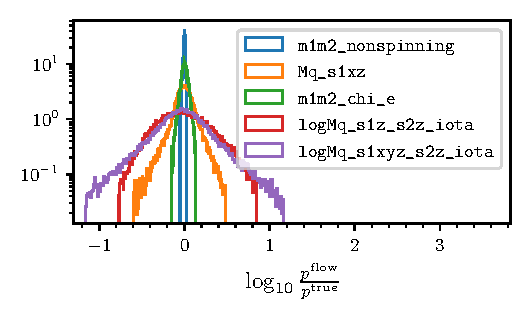
\includegraphics[scale = 1.]{flow_validation}
	\caption{WRITEME}
	\label{fig:flow_validation}
\end{figure}


\begin{table}
	\begin{tabular}{c c c c} 
	 %\hline
	 \phantom{manifold} & Parameter space & $D$ & Architecture \\ 
	 \toprule
	 \texttt{m1m2\_nonspinning} &
	 	\begin{tabular}{@{}l@{}} $m_1,m_2\in [1, 200] \mathrm{M_\odot}$ \\ $q\in [1,30]$ \\ $f \in [15, 1024] \SI{}{Hz}$ \\
	 	\texttt{IMRPhenomD} \cite{Khan:2015jqa} \end{tabular} & 2 & 60 60 30\\
 	\addlinespace[3pt]
 	\cdashline{1-4}
 	\addlinespace[3pt]
	 \texttt{Mq\_s1xz} & 
	 	\begin{tabular}{@{}l@{}} $M\in [25, 100] \mathrm{M_\odot}$ \\ $q\in [1,5]$  \\ $s_1\in [0, 0.99]$  \\ $\theta_1 \in [0, \pi]$  \\ $f \in [15, 1024] \SI{}{Hz}$\\
	 	\texttt{IMRPhenomXP} \cite{Pratten:2020ceb} \\ \end{tabular} & 4 & 70 70\\
 	\addlinespace[3pt]
	\cdashline{1-4}
	\addlinespace[3pt]
	 \texttt{m1m2\_chi\_e} & 
		\begin{tabular}{@{}l@{}} $m_1,m_2\in [1, 50] \mathrm{M_\odot}$ \\ $q\in [1,20]$  \\ \chi \in [-0.99, 0.99] \\ $e\in [0, 0.5]$ \\  $f \in [10, 1024] \SI{}{Hz}$ \\ \texttt{EccentricFD} \cite{lalsuite} \\ \end{tabular} & 4 & 60 60 60\\
	\addlinespace[3pt]
	\cdashline{1-4}
	\addlinespace[3pt]
		\begin{tabular}{@{}c@{}}
			\texttt{logMq\_s1z\_s2z\_iota} \\ (with HM) \\
		\end{tabular} & 
	 	\begin{tabular}{@{}l@{}} $m_1,m_2\in [50, 300] \mathrm{M_\odot}$ \\ $M\in [100, 400] \mathrm{M_\odot}$ \\ $q\in [1,10]$  \\ $s_{1z},s_{2z}\in [-0.99, 0.99]$  \\ $\iota \in [0, \pi]$  \\ $f \in [10, 1024] \SI{}{Hz}$\\
	 	\texttt{IMRPhenomXP} \cite{Pratten:2020ceb} \\ \end{tabular} & 5 & 20 60 60\\
 	\addlinespace[3pt]
	\cdashline{1-4}
	\addlinespace[3pt]
		\texttt{logMq\_s1xyz\_s2z\_iota} &
	 	\begin{tabular}{@{}l@{}} $m_1,m_2\in [1, 100] \mathrm{M_\odot}$ \\ $M\in [2, 150] \mathrm{M_\odot}$ \\ $q\in [1,20]$  \\ $s_1\in [0, 0.99]$  \\ $\theta_1 \in [-\pi, \pi]$ \\ $\phi_1 \in [0, \pi]$ \\ $s_{2z}\in [-0.99, 0.99]$  \\ $\iota \in [0, \pi]$  \\ $f \in [15, 1024] \SI{}{Hz}$\\ \texttt{IMRPhenomXHM} \cite{Garcia-Quiros:2020qpx} \\ \end{tabular} & 7 & 100 60 60 60\\
	 \bottomrule
	\end{tabular}
	\caption{WRITEME}
	\label{tab:flow_validation}
\end{table}

\begin{figure}[t]
	\centering
	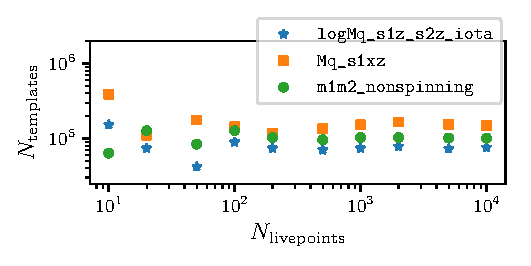
\includegraphics[scale = 1.]{template_placement_validation}
	\caption{WRITEME}
	\label{fig:template_placement_validation}
\end{figure}

	%%%%%%%%%%%%%%%%%%%%%%%%%%%%%%%%%
\section{Validation} \label{sec:validation}

In this section, we assess the performance of the two key ingredients of our template bank generation algorithm, namely the normalizing flow model and the random placement algorithm.
Our goal is to understand the limitations of our algorithm as well as to make an informed choice of the various hyperparameters that impact the quality of the template bank.

In our experiments, we will consider different manifolds, which will be named with a string that lists the manifold coordinates. The coordinates are grouped by mass coordinates, spin coordinates, (eventual) eccentricity coordinates (i.e. eccentricity and mean anomaly) and (eventual) angles coordinates (i.e. inclination and reference phase).
A manifold string has the format \texttt{Masses\_Spin1\_Spin2\_Eccentricity\_Angles}.
Valid options for the mass coordinates are \texttt{m1m2}, which uses $m_1$ and $m_2$ as coordinates, \texttt{Mq}, which uses total mass $M = m_1+m_2$ and mass ratio $q = m_1/m_2 >1$, and \texttt{logMq}, using $\log_{10}M$ instead of $M$.
Simirarly, other variables are listed by their names.
The spin coordinate \texttt{chi} uses the effective spin parameter $\chi$, setting $s_\text{1z} = s_\text{2z} = \chi$ and all the other spin compoenents to $0$.

If more than one spin coordinate is given for a given BH, the spin vector $\mathbf{s}$ will be parametrized in spherical coordinates with magnitude $s \in [0,1)$ and angles $\theta \in [-\pi,\pi]$ and $\varphi \in [0, \pi]$ as follow:
%
\begin{align}
	s_\text{x} & = s \sin\theta \cos\phi \\
	s_\text{y} & = s \sin\theta \sin\phi \\
	s_\text{z} & = s \cos\theta
\end{align}
%
Note that the angle $\theta$ quantifies the amount of precession: with $\theta = 0, \pm \pi$ the spin has only a z component (i.e. is aligned to the orbital angular momentum), while for $\theta = \pi/2$ there is maximal precession, as the spin vector only has an in-plane component.

\subsection{Normalizing flow validation} \label{sec:flow_validation}

To study the accuracy of the normalizing flow model in reproducing the volume element of the parameter space, we consider five manifolds. The manifolds are reported in Tab.~\ref{tab:flow_validation} together with the region of the parameter space they cover. We also report the waveform approximant used to compute the metric as well as the frequency range where the metric is computed.
The manifold were chosen to have a variety of number of dimensions $D$ and to cover a broad ranges of physical scenarios (precession, HM and eccentric orbits).

For each manifold we generate a dataset of $3\times 10^5$ points and we compute the (log) value of the PDF Eq.~\eqref{eq:pdf_uniform}. We then train a normalizing flow model on each of the datasets.
The architecture of each flow is also reported in Tab.~\ref{tab:flow_validation}.

In Fig.~\ref{fig:flow_validation} we report a histogram with the accuracy of the normalizing flow reconstruction of the PDF on each manifold. This is quantified by $\log_{10}\frac{p^\mathrm{flow}}{p^\mathrm{true}}$, which measures the logarithmic ratio between the two PDFs.

Overall, the accuracy of the flow is (almost) always contained within one order of magnitude: whether this error is acceptable for the purpose of template placement needs to be assessed on a case-by-case basis.

We note that all histograms are well centered around $0$, showing that the flow does not have any sistematic bias. Moreover, the accuracy tends to be higher for low dimension manifold. Indeed, low dimensional manifolds present an easier learning task for the flow.

The manifold \texttt{logMq\_s1xyz\_s2z\_iota} has by far the worst performance (indeed its the largest dimension manifold being considered). However, we stress that it parametrize a huge parameter space, which can't be realistically covered by a template bank. Hence, as a realistic bank on the manifold will necessarily cover a subset of it, a flow trained on that smaller parameter space will most certainly show better accuracy, since it will face an easier regression task.

Finally, we see that the flow trained on the eccentric manifold \texttt{m1m2\_chi\_e} has remarkably good performance. This can be explained by the fact that the approximant \texttt{EccentricFD} \cite{lalsuite} used is analytical. This makes sure that it has a very smooth behaviour across the parameter space, which can be easier to learn by the normalizing flow model.


\subsection{Template placement performance} \label{sec:template_placement}

As already remarked, the template placement method in use closely matches the one introduced in \cite{Coogan:2022qxs}.
The main novelty introduced here is sampling with the normalizing flow, as opposed to rejection sampling.

For the random placement method, there are two parameters to tune that affect the final bank size. They are the number of livepoints $N_\text{livepoints}$ and the covering fraction $\eta$.
The authors of \cite{Coogan:2022qxs} make an extensive study on how the bank size depends on such quantities and recommend setting $\eta = 0.9$ and $N_\text{livepoints} = 1000$. We do not repeat such in-depth studies here.

We limit ourselfs to study the convergence of the template number $N_\text{templates}$ as a function of $N_\text{livepoints}$ (see \cite[Fig.~4 (right)]{Coogan:2022qxs}, in the case of manifolds with precessing and HM signals.
For the study, we chose the manifolds \texttt{m1m2\_nonspinning}, \texttt{Mq\_s1xz} and \texttt{logMq\_s1z\_s2z\_iota} introduced in Sec.~\ref{sec:flow_validation} (see also Tab.~\ref{tab:bank_comparison}). The second manifold covers a precessing parameter space, while the metric on the latter manifold is computed with an HM approximant.
We present our results in Fig.~\ref{fig:template_placement_validation}, where the number of template is computed with a covering fraction $\eta = 0.9$ with a varying $N_\text{livepoints}$.

In all cases the number of templates converges to a constant value as $N_\text{livepoints}$ increases. Already $\sim 500$ livepoints are enough to provide an accurate estimation of the bank size.
Our results closely match the findings of \cite{Coogan:2022qxs}, expanding them to higher dimensional manifolds and to larger template banks.

\stefano{Where do we put some timing numbers??? We just need the orders of magnitude...}

\section{Comparison with other bank generation methods} \label{sec:other_methods}

In this section we compare the banks generated by \texttt{mbank} with two banks available in the literature generated with two different methods.
The first bank we consider is a non-spinning HM bank \cite{Harry:2017weg}, covering the high mass region of the BBH parameter space. The bank was generated using the stocastic placement algorithm, as implemented in the code \texttt{sbank} \cite{Ajith:2012mn}.
The second bank is the non-precessing spinning bank \cite{Sakon:2022ibh} in use by the \texttt{GstLAL} pipeline \cite{PhysRevD.95.042001, gstlal_paper2} during the Fourth Observing run. It was generated using a metric template placement algorithm called \texttt{manifold} \cite{Hanna:2022zpk} and it covers a very wide mass range in the BBH and BNS parameter space.
Both banks have a minimum match requirement $MM$ of $0.97$.

In much of what follows we will need to measure the coverage of a bank. To do so, we randomly extract a number of signal templates, usually called {\it injections}, and we construct the signal at the interferometer ${s = F_+h_+ + F_\times h_\times}$.
For each injection at a given point on the manifold $\theta$, we compute the fitting factor $FF$, defined as the minimum match the injection has with the templates of the bank:
\begin{equation}\label{eq:FF}
	FF(\theta) = \max_{\theta^\prime \in \text{bank}} \mathcal{M}(\theta, \theta^\prime)
\end{equation}
Clearly, the match is computed using Eq.~\eqref{eq:symphony_snr}.

Studying the statical properties of the fitting factor on a large set of injections is a standard procedure to characterize the properties of a template bank, virtually used to validate any template bank in the literature.

\begin{table}
	\begin{tabular}{c c c c} 
	 \hline
	 \phantom{Name} & Parameter space & \multicolumn{2}{c}{
		\begin{tabular}{c c} \multicolumn{2}{c}{Size}  \\ Original & \texttt{mbank} \\ \end{tabular}	 
	 } \\ 
	 \toprule
	 HM bank \cite{Harry:2017weg} & \begin{tabular}{@{}l@{}} $M\in [50, 400] \mathrm{M_\odot}$ \\ $q\in [1,10]$  \\ $\iota\in [0,\pi]$ \\ $\varphi\in [0,2\pi]$   \\ \end{tabular} & 20500 & 58932 \\
 	\addlinespace[3pt]
	\cdashline{1-4}
	\addlinespace[3pt]
	 \texttt{GstLAL} O4 bank \cite{Sakon:2022ibh} & \begin{tabular}{@{}l@{}} $m_1,m_2\in [1, 200] \mathrm{M_\odot}$ \\ $q\in [1,20]$  \\ $\chi\in [-0.99,0.99]$   \\ \end{tabular} & $1.8 \times 10^6$  & $1.3 \times 10^6$  \\
	 \bottomrule
	\end{tabular}
	\caption{WRITEME}
	\label{tab:bank_comparison}
\end{table}

\begin{figure}[t]
	\centering
	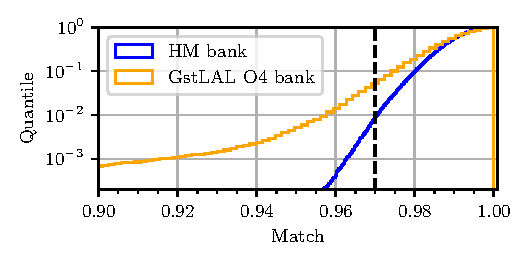
\includegraphics[scale = 1.]{test_banks_hist}
	\caption{WRITEME}
	\label{fig:test_banks_hist}
\end{figure}
\begin{figure*}[t]
	\centering
	\begin{subfigure}[t]{0.49\textwidth}
		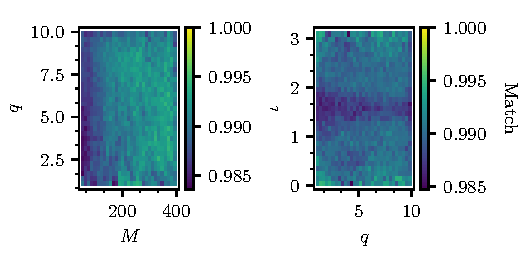
\includegraphics[scale = 1.]{symphony_HM_injections}
		\caption{Nonspinning HM bank \cite{Harry:2017weg}}
		\label{fig:symphony_HM_injections}
	\end{subfigure}
	\hfill
	\begin{subfigure}[t]{0.49\textwidth}
		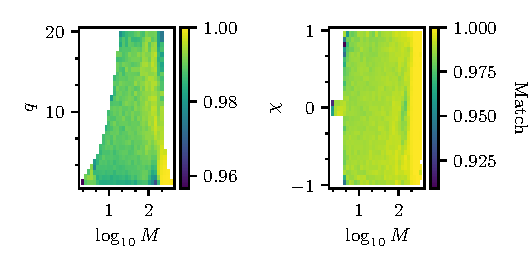
\includegraphics[scale = 1.]{bank_O4_injections}
		\caption{All sky bank \cite{Sakon:2022ibh}}
		\label{fig:bank_O4_injections}
	\end{subfigure}
	\caption{WRITEME}
\end{figure*}

%\begin{figure}[t]
%	\centering
%	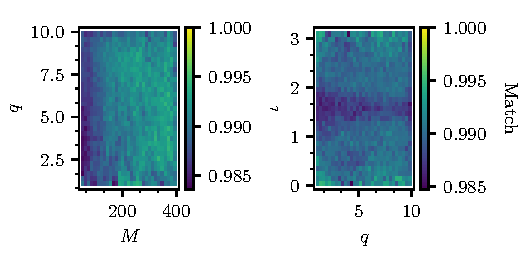
\includegraphics[scale = 1.]{symphony_HM_injections}
%	\caption{WRITEME}
%	\label{fig:symphony_HM_injections}
%\end{figure}

%\begin{figure}[t]
%	\centering
%	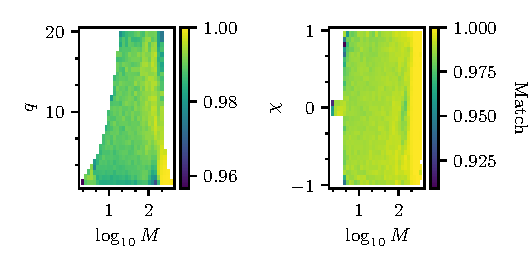
\includegraphics[scale = 1.]{bank_O4_injections}
%	\caption{WRITEME}
%	\label{fig:bank_O4_injections}
%\end{figure}

\subsection{A non spinning HM template bank} \label{sec:HM_comparison}

The non spinning HM bank described in \cite{Harry:2017weg} covers systems with total mass $M$ in the range $[50, 400] \mathrm{M_\odot}$ and mass ratio $q\in [1,10]$. It also includes the inclination angle $\iota$ and reference phase $\varphi$ of the system, both covering the whole possible spectrum of values $\iota\in [0,\pi]$ and $\varphi\in [0,\pi]$.
The authors use the PSD \cite{} and consider a low frequency cutoff $f_\text{min} = \SI{10}{Hz}$.

As already noted, they use the state-of-the-art code \texttt{sbank} \cite{Ajith:2012mn, PhysRevD.80.104014}. New template are randomly drawn from a sutiable distribution (designed to roughly approximate Eq.~\eqref{eq:pdf_uniform}). For each potential new template, called {\it proposal}, it is computed the match against all the templates already added to the bank. If the maximum match of the proposal is smaller than the minimum match requirement, the new template is added to the bank. This method is very accurate and it is known to provide effective coverage with a low number of template. Of course, this comes at a large computational cost.

We reproduce the non spinning HM bank with our code. We place templates on the manifold \texttt{logMq\_nonspinning\_iotaphi}, with coordinates $\log_{10}M$, $q$, $\iota$ and $\varphi$. We use the same PSD and coordinate ranges of the original bank.
We train a normalizing flow model with $4$ layers each with $60, 60, 60, 10$ hidden features and we choose $N_\text{livepoints} = 2000$ and a covering fraction $\eta = 0.8$.
Our bank has $58932$ templates, while the original bank is reported to have $20500$.
Such information are summarized in Tab.~\ref{tab:bank_comparison}.
We perform an injection study, drawing $10^5$ injections uniformly from the manifold. The results of such study are reported in Fig~\ref{fig:test_banks_hist} and Fig~\ref{fig:symphony_HM_injections}.

First of all, we note that our bank successfully covers the parameter space, with only $1\%$ of the injection with fitting factor below $0.97$ and less than $1\textperthousand$ with fitting factor below $0.96$. Such figures are very similar to those reported in \cite{Harry:2017weg}.
In Fig.~\ref{fig:symphony_HM_injections}, we observe that the coverage is uniform across the space, i.e. we do not see regions where the fitting factor is significantly different from the others.

Comparing the number of templates, it is striking that our bank has almost three times more templates than the original template bank.
As no template rejection is done during the random bank construction, there is no control over templates being too close to each other. For this reason, an overcoverage of the space is inherent to the random template placement and it was also reported in \cite{Messenger:2008ta,Coogan:2022qxs}.

\subsection{A template bank for O4} \label{sec:all_sky_comparison}

The non-spinning bank (with no HMs) introduced in \cite{Sakon:2022ibh} covers a broad mass range, with systems with component masses $m_1, m_2 \in [1,200] \mathrm{M_\odot}$. The spins of the two objects are constrained to be equal to each other, $s_\text{1z} = s_\text{2z} = \chi$ and they span the range $[-0.99, 0.99]$.
The authors impose a upper limit to the mass ratio $q<20$. Moreover, for objects with component mass $m<3  \mathrm{M_\odot}$ they limit the effective spin $chi$ to the range $[-0.05, 0.05]$\footnote{This is motivated by astrophysical considerations. Objects with masses smaller than $3  \mathrm{M_\odot}$ are likely to be Neutron Stars and such objects are believed to develop only mild rotations.}.
The authors use the O4 Design PSD \cite{} and consider a low frequency cutoff $f_\text{min} = \SI{10}{Hz}$.

The comparison with \cite{Sakon:2022ibh} is particularly interesting, since the bank is also done with a metric template placement, implemented in the \texttt{manifold} code \cite{Hanna:2022zpk}. \texttt{manifold} uses a geometric approach, where the parameter space is iteratively split into (hyper)rectangles along the coordinates, until the volume of each rectangle reaches a sufficiently small value that it can be covered by a single template.

Our bank matches \cite{Sakon:2022ibh} in the parameter space and other choices and covers the manifold \texttt{m1m2\_chi}, sampling the coordinates $m_1$, $m_2$ and $\chi$. This is summarized in Tab.~\ref{tab:bank_comparison}.
To generate our bank, we trained three different normalizing flows in different regions of the parameter space. A first normalizing flow covers the BBH region with $m_1 \in [3,200] \mathrm{M_\odot}$, with $\chi \in [-0.99, 0.99]$. A second one takes care of the BNS region, covering the manifold, ${(m_1, m_2, \chi) \in [1,3]\mathrm{M_\odot}\times[1,3]\mathrm{M_\odot}\times [-0.05, 0.05]}$.
A third normalizing flow specializes in the high mass region, characterized by $m_1, m_2 \in [100,200] \mathrm{M_\odot}$. In this region, the template density is so low, that hardly any template is placed by the first normalizing flow, hence the need for additional coverage.
All the normalizing flow models are made of $5$ layers of $10$ hidden features each.
Three templates banks are generated using each normalizing flow and they are merged together afterwards.
For the template placement we set $N_\text{livepoints} = 2000$ and covering fraction $\eta = 0.95$.
The resulting bank has $1326805$ templates.

To validate our bank, we generate an injection set with $10^5$ injections, with masses uniformly sampled in $\log_{10}$.
Results of our injections studies are reported in Fig~\ref{fig:test_banks_hist} and Fig~\ref{fig:bank_O4_injections}.

In Fig~\ref{fig:test_banks_hist}, we see that $\sim 5\%$ of the injections has a match below $0.97$. The low fitting factor injections are mostly located around the low mass corners of the bank, clustered on the low mass end of the BNS region and in the high spin - low mass edge of the BBH region.
Inside the template bank and on the high mass end of the parameter space, satisfactory coverage is achieved.
Our results suggest that \texttt{mbank} struggles to accurately cover the boundaries of the parameter space. This problem has been observed also with other placement methods \cite{} and several strategies have been proposed \cite{} to cope with it. Within our framework, the simplest option would be to extend the boundaries of the bank at low masses, thus ensuring better coverage of the region of interest.
%\stefano{Cite some shit here!!}

With slight variations depending on the region of parameter space, \cite{Sakon:2022ibh} report that $10\%$ of BBH injections are have fitting factor smaller than $\sim 0.98$, while for our bank the $10^\text{th}$ percentile is around $0.975$.
Even though these figures are difficult to compare due to different injection sets, it seems fair to state that, compared to \cite{Sakon:2022ibh}, our template bank provides slightly worse injection recovery.
On the other hand, our template bank has $30\%$ {\it less} templates, matching the number of templates placed by \texttt{sbank} in the same region \cite{Sakon:2022ibh}. With an accurate treatment of the boundaries, the coverage of our template bank will easily match the one of \cite{Sakon:2022ibh}, with a comparable bank's size.

%%%%%%%%%%%%%%%%%%%%%%%%%%%%%%%%%%%%%%
\begin{figure*}[t]
	\centering
	\begin{subfigure}[t]{\textwidth}
		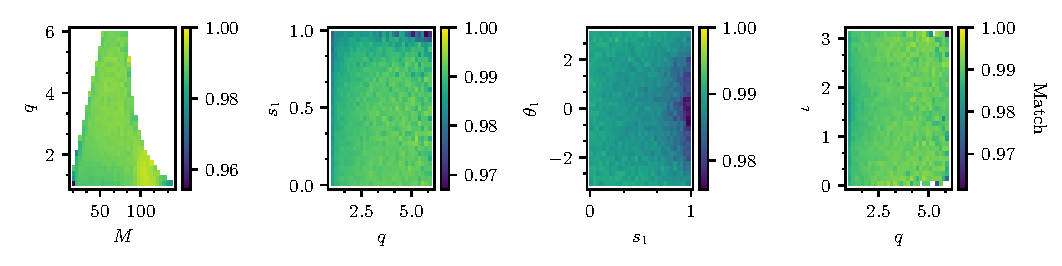
\includegraphics[scale = 1.]{precessing_injections}
		\caption{Fitting factors}
	\end{subfigure}
	\begin{subfigure}[t]{\textwidth}
		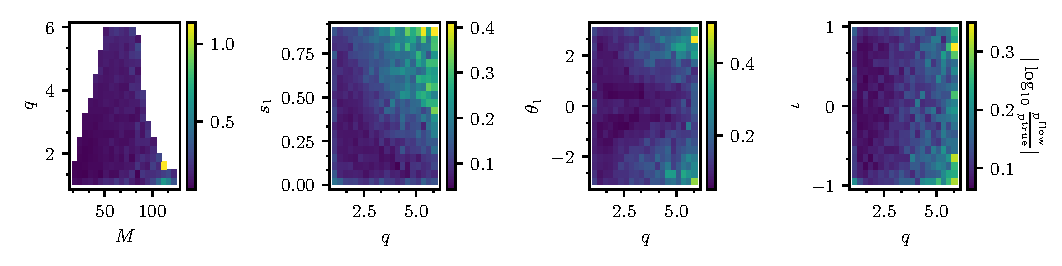
\includegraphics[scale = 1.]{precessing_flow_accuracy}
		\caption{Flow accuracy}
	\end{subfigure}
	\caption{WRITEME}
	\label{fig:precessing_injections}
\end{figure*}

%\begin{figure*}[t]
%	\centering
%	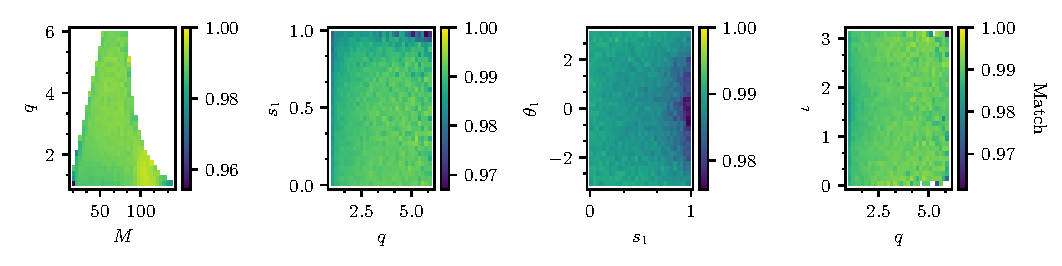
\includegraphics[scale = 1.]{precessing_injections}
%	\caption{WRITEME}
%	\label{fig:precessing_injections}
%\end{figure*}

\begin{figure}[t]
	\centering
	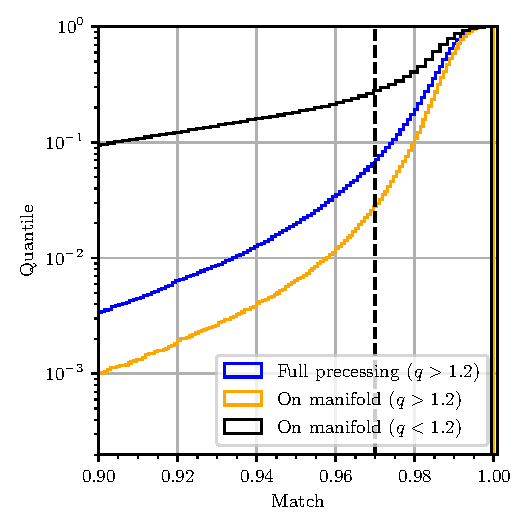
\includegraphics[scale = 1.]{precessing_hist}
	\caption{WRITEME}
	\label{fig:precessing_hist}
\end{figure}


\begin{figure}[t]
	\centering
	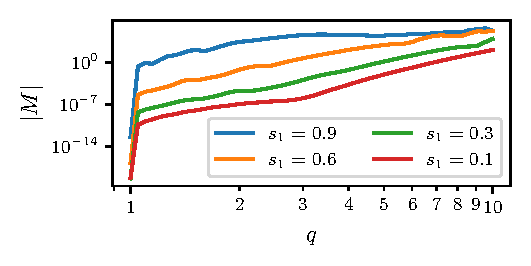
\includegraphics[scale = 1.]{metric_det_vs_q}
	\caption{WRITEME}
	\label{fig:metric_vs_q}
\end{figure}


%%%%%%%%%%%%%%%%%%%%%%%%%%%%%%%%%%%%%%

\section{Novel applications of the method} \label{sec:novel_applications}

Our template placement method allows for several exciting applications in GW data analysis.
Obviously, the most straighforward one is the generation of a precessing template bank and of a HM bank. While in principle it is possible to generate them with stochastic placement, very few of such banks have been generated so far, mostly due to the enourmous computational cost of choosing the right parameter space and of placing the templates. Their generation becomes feasible thanks to \texttt{mbank}.

Besides efficient high dimensional bank generation, our method can be used for other different purposes. They include choosing the appropriate parameter space to cover by forecasting the size of a bank or selecting the appropriate coordinates to cover a given region of binary systems. Moreover, our normalizing flow might be used as a proposal for stochastic placement algorithm or even for parameter estimation \cite{Veitch:2014wba}.

In what follows, we generate a large precessing template banks and a large spinning (non-precessing) HM bank. Moreover, we discuss with some details other novel applications of our code.

\subsection{A precessing bank} \label{sec:precessing_bank}

\subsubsection{Choosing the parameter space}

The main difficulty to generate a precessing bank lies in the huge size of the parameter space. As we will show below in more details, a precessing bank can easily have {\it billions} of templates, even when covering the mass range routinely explored by standard non-precessing searches. As standard search pipeline can handle only up to a few {\it millions} templates, due to computational cost, the bank size plays a crucial role in the selection of a suitable parameter space, setting very stringent constraints on the feasible regions to explore with a GW search.

Another difficulty, somehow related to the first one, arises from the choice of the BBH coordinates to include in the bank, i.e. on the choice of manifold.
In principle, to precessing BBH is described by $10$ parameters (two masses, six spins and two angles). However, some of them are irrelevant (i.e. they don't affect too much the waveform) and including them in the bank does not produce any sensible improvement.
On top of this, there are concerns about the validity of the metric approximation of the match (see also Sec.~\ref{sec:other_applications}), which might loses its predictivity in presence of an irrelevant coordinate in the parameter space. Indeed, an irrelevant coordinate $i$ implies that $\partial_i h \simeq 0$. This means that the metric has at least one zero eigenvalues, with great harm to the metric predictivity.

Finally, a more technical complexity arises from the fact in high dimensional spaces both the training of a normalizing flow (see Sec.~\ref{sec:flow_validation}) and the template placement become harder, hence possibly harming the effectualness of the template bank.

All such difficulties imply that great care must be taken when deciding both the parameter space and the BBH variables to include in the bank.
The choices are entangled, since covering different manifolds with the same mass range can produce banks of very different sizes.

Of course, when choosing a manifold there is a trade between the effectualness of the full $10$ dimensional precessing space and the size of the bank. Roughly speaking, choosing a lower dimensional sub-manifold reduces the bank size, at the cost of a loss in the bank's effectualness across the full space.
Here the theory comes handy. In \cite{Schmidt:2014iyl}, the authors find that the effect of the four in plane spin components (i.e. $s_\text{1x}, s_\text{1y}, s_\text{2x}, s_\text{2y}$) can be well approximated by a single precessing spin parameter $\chi_P$ assigned to x-component of the heavies object's spin.
Thus, a generic precessing system is roughly equivalent to a system with $\mathbf{s}_\text{1} = (\chi_P, 0, s_\text{1z})$ and $\mathbf{s}_\text{1} = (0, 0, s_\text{2z})$, effectively creating an explicit mapping between a six dimensional spin manifold to a three dimensional one.
In a later work \cite{Thomas:2020uqj}, it is suggested that to capture the combined effect of precession and HM, a two dimensional spin parameter $\vec{\chi_P}$ is needed. In this case, the mapping is between  a six dimensional spin manifold to a four dimensional one.

Both works suggest that the in plane components of the spin on the lightest object (i.e. $s_\text{2x}, s_\text{2y}$) can be neglected, highly reducing the dimensionality of the parameter space.
Moreover, since we are not concerned with precession combined with HM\footnote{In such space, the template banks would be unfeasibly large!}, we can rely on the one dimensional effective spin mapping \cite{Schmidt:2014iyl} to also neglect the y-component of the spin of the heaviest object.

We then consider only three out of six spin components, $s_\text{1x}, s_\text{1z}$ and $s_\text{2z}$, where all the effects of precession are included in $s_\text{1x}$. To obtain accurate coverage we are also forced to inclue the inclination $\iota$ in the manifold. Some investigations showed that reference phase $\varphi$ makes the template placement really hard, hence forcing us to neglect $\varphi$. Luckily, injections studies show that this doesn't harm too much the bank's ability to cover the space. This might not be the case for precession combined with HMs.

To summarize, we find that the $6$ variables $M$, $q$, $s_\text{1x}$, $s_\text{1z}$, $s_\text{2z}$ and $\iota$ satisfactorily match most of the precessing signals in a ten dimensional space.
This claim is confirmed by an injection study Fig.~\ref{fig:precessing_hist}.
A precessing template bank with HM will probably need to sample two more variables $s_\text{1y}$ and $\varphi$, hence increasing the dimensionality to $8$.

About the parameter space, we are interested to target BBHs where precession is stronger: such systems are most likely to be missed by current non-precessing searches \cite{}.
Precession is more visibile for high mass ratio systems and for high values of spins. Moreover, as more cycles are detectable, precessing effect will be stronger for longer signals due to the accumulation of the phasing effects of precession.
The considerations above point towards searching for very asymmetric low mass systems, hence the Neutron Start Black Hole (NSBH) woud be an ideal target for a precessing bank. However, as shown below in Sec.~\ref{sec:other_applications} covering the NSBH region is unfeasible, as hundreds of millions of templates would be needed.
For this reason, we fall back to a different, less extreme region of the parameter space. After several investigations, made possible by the speed and flexibility of our approach, we found that a parameter space with component masses in the range $[8, 70] \mathrm{M_\odot}$, with a mass ratio cut-off of $6$, produces a bank with feasible size.
Such range is large enough to encompass most of the GW detections made so far \cite{LIGOScientific:2020kqk, KAGRA:2021duu}, hence we likely maximise our detection probability (if precessing systems exists in such mass ranges).
We obtain a precessing bank with $\sim 2 \text{millions}$ templates. Extending the parameter space to lower masses results in a much larger banks, which current pipelines are unable to process.

In closing, we stress that all the investigation reported above would not have been possible without our method. Indeed, a fast template bank generation across different manifold and regions of parameter space is crucial to obtain invaluable pieces of information quickly. With slower template placement methods, the bank generation time would be too long to carry on any of the investigations we made.

\subsubsection{Generating and validating the bank}

As discussed above, we place the templates for our precessing bank on the manifold \texttt{logMq\_s1xz\_s2z\_iota}, with coordinates $\log_{10}M$, $q$, $s_\text{1}$, $\theta_\text{1}$, $s_\text{2z}$ and $\iota$.
We consider BBHs with individual masses between  $8$ and $70 \mathrm{M_\odot}$, with a maximum mass ratio $q = 6$.
The other quantities are set on the largest allowed range.

To compute the metric, we use the Advanced LIGO O4 sensitivity estimate and we set a frequency range of $[15, 1024] \SI{}{Hz}$.
We train a normalizing flow with $3$ layers with $100$, $100$ and $60$ hidden features respectively, using a dataset of $4\times 10^5$ points.
The flow performance after training is reported in Fig.~\ref{fig:HM_flow}.
To generate the bank, we use a minimum match requirement of $0.97$, with a covering fraction $\eta = 0.9$, estimated with $3000$ livepoints.
We obtain a bank with $1669683$ templates.
The bank generation took a few hours in total: $~\SI{2}{hours}$ for the dataset generation, $\sim \SI{30}{minutes}$ for the training of the flow and $\sim \SI{5}{minutes}$ for the template placing. This is a fraction of the time required to generate a similar bank with the state-of-the-art stochastic algorithm.

To study the performance of our template bank, we generate two injections sets, with masses sampled uniformly in $\log m_1$ and $\log m_2$.
The first set, labeled ``Full precessing" has fully precessing injections (with two $3D$ spins and varying $\varphi$). The second one, denoted as ``On manifold", has injections only lying on the manifold \texttt{logMq\_s1xz\_s2z\_iota}, thus covering only a subset of the ``Full precessing" set.
The latter set is needed to asses the coverage of the bank on the manifold the templates lie on and thus is a measure of how accurate is the placement of the templates.
On the other hand, the ``Full precessing" injection set evaluates the ability of the bank to recover a generic precessing signal, hence assessing the quality of our choice of manifold.
Clearly, a fully precessing search will be mostly interested in the fitting factor obtained with first injection set.

We report the results of our study in Fig~\ref{fig:precessing_hist}, in the form of a histogram of the fitting factors, and in Fig.~\ref{fig:precessing_injections}, where we study the dependency of the fitting factor across the parameter space.
As clear from Fig~\ref{fig:precessing_hist}, the bank provides a unsatisfactory coverage for the $q\sim 1$ region, where $q \lessapprox 1.25$, with only $77\%$ of the injections ``On manifold" having a fitting factor higher than $0.97$. The problem is more severe for high values of $s_1$.
On the other hand, for systems with mass ratio $q \gtrapprox 1.25$, the template bank provides a good coverage: $98\%$ of the injections ``On manifold" has a fitting factor large than $0.97$.

The low performance at low mass ratio can be explained by looking at Fig.~\ref{fig:metric_vs_q}, where we plot $|M|$ as a function of $q$ keeping constant the all the other coordinates. We observe that for $q \sim 0$ the metric determinant goes rapidly to $0$. This means that the placing algorithm places very few templates in the $q\sim 1$ region, possibly undercovering drastically the space. On the other hand, the metric has the same behaviour even for non-precessing signals and this raises the obvious question of why we don't see a similar issue in the O4 template bank. The reason for this needs more investigation, but this might be due to the higher dimensionality of the space, which makes the placement harder.

The lack of coverage for $q\sim 1$ should not be of concern for the effectivness of the bank in a real search scenario. Indeed, precession for $q\sim 1$ has very little effect on the BBH waveform, hence a precessing system with symmetric masses is likely to be detected by current template banks.

In Fig.~\ref{fig:precessing_injections}, we note that the coverage is rather uniform across the parameter space. The median fitting factor drops significantly for the maximally precessing region, where $q \simeq 6$ and $s_1 \simeq 1$ and $\theta_1 \simeq 0$ (that means $s_\text{1x} \simeq 1$ and $s_\text{1z} \simeq 0$).
This can be explained by noting that the region is at the boundaries of the parameter space, with all the difficulties in template placement already discussed. More importantly, the flow performance degrades in that undercovered corner of the space: the true template density $\sqrt{|M|}$ might be understimated by the normalizing flow, which accordingly places less templates than optimal.

The fitting factor of the ``Full precessing" injection set is fairly good, with only $6\%$ of the injections below the target match. This means that the $\chi_P$ approximation that motivates our choice is robust: the manifold \texttt{logMq\_s1xz\_s2z\_iota} provides a faithful low dimensionality representation of the entire precessing parameter space.

\stefano{Maybe the threshold can be 1.2 or even 1.1?? If you do the bank again, think about this...}


%%%%%%%%%%%%%%%%%%%%%%%%%%%%%%%%%%%%%%
\begin{figure*}[t]
	\centering
	\begin{subfigure}[t]{\textwidth}
		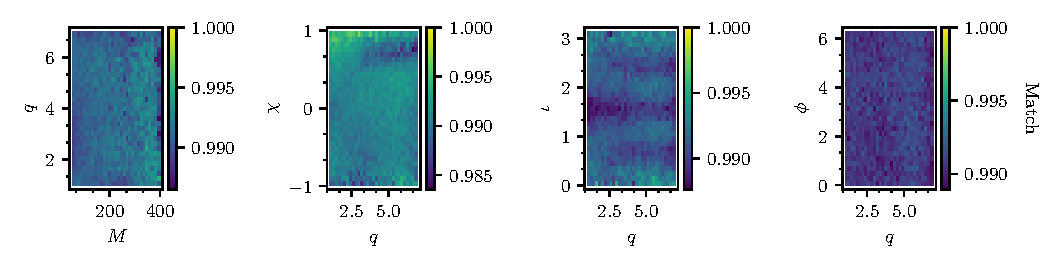
\includegraphics[scale = 1.]{HM_injections}
		\caption{Fitting factors}
		\label{fig:HM_fitting_factor}
	\end{subfigure}
	\begin{subfigure}[t]{\textwidth}
		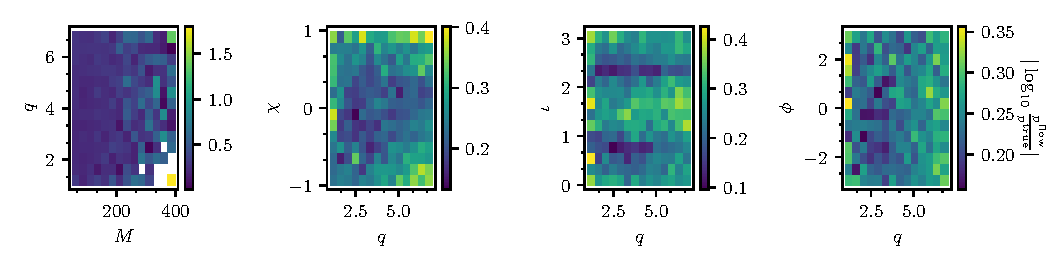
\includegraphics[scale = 1.]{HM_flow_accuracy}
		\caption{Flow accuracy}
		\label{fig:HM_flow}
	\end{subfigure}
	\caption{WRITEME}
	\label{fig:HM_injections}
\end{figure*}

%\begin{figure*}[t]
%	\centering
%	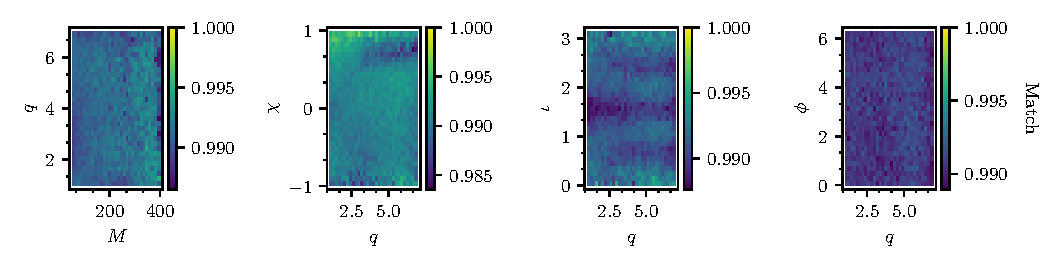
\includegraphics[scale = 1.]{HM_injections}
%	\caption{WRITEME}
%	\label{fig:HM_injections}
%\end{figure*}

\begin{figure}[t]
	\centering
	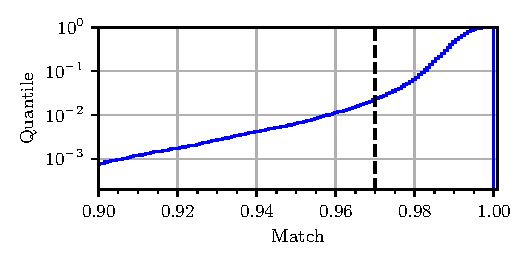
\includegraphics[scale = 1.]{HM_hist}
	\caption{WRITEME}
	\label{fig:HM_hist}
\end{figure}
%%%%%%%%%%%%%%%%%%%%%%%%%%%%%%%%%%%%%%

\subsection{A spinning HM bank} \label{sec:HM_spinning_bank}

In a sense, non-precessing HM template banks are easier to generate than precessing ones, due to a smaller dimensionality of the HM parameter space. Indeed, a generic non-precessing binary system is characterized by $6$ parameters (two masses, two spins and two angles) but, as for the non-HM case, the spin can be easily parametrized with an effective spin parameter, reducing the number of dimensions to $5$.
There are still severe contraints related to the bank size, hovewer they are easier to deal with, since they are not coupled to uncertainties to the choice of manifold.
Nevertheless, some investigation is still required to find a parameter space that can be feasibly covered.

We used \texttt{mbank} to generate an HM aligned spin bank, covering the high mass region of the BBH parameter space.
High mass events are notoriously hard to detect \cite{LIGOScientific:2021tfm, Chandra:2021wbw}. As they are very short, their morphology matches closely those non-gaussian transient noise bursts, also called {\it glitches}, \cite{Blackburn:2008ah, Zevin:2016qwy, LIGOScientific:2016gtq}. In this scenario, a more realistic model for the waveform can improve the detectability of such signals, thanks to both an increase in recovered SNR and to a more accurate signal-based veto \cite{Babak:2005kv, PhysRevD.95.042001}.

Our HM bank covers the manifold \texttt{logMq\_chi\_iotaphi}, sampling $\log_{10}M$, $q$, the effective spin parameter $\chi$ as well as inclination and reference phase.
We consider templates with total mass $M$ between $50 \mathrm{M_\odot}$ and $400 \mathrm{M_\odot}$ and a mass ratio smaller than $7$. The spin lies in range $[-0.99, 0.99]$ and, as usual, $\iota \in [0, \pi]$ and $\varphi \in [-\pi, \pi]$.

We generate a dataset with $4\times 10^5$ points and we train a normalizing flow with $4$ layers, each with $n_\text{hidden} = 60$ hidden features. The accuracy of the normalizing flow is reported in Fig.~\ref{fig:HM_flow}.
For the template placement, we use a minimum match requirement of $0.97$ and we set a covering fraction $\eta = 0.8$, estimated with $10000$ livepoints.
The overall bank gathers $2115299$ templates.
The bank generation took roughly the same time as for the precessing bank.

We study the bank performance with $10^5$ injections and we report their fitting factor in Fig.~\ref{fig:HM_fitting_factor} and Fig.~\ref{fig:HM_hist}.
Our injection study show that the only $\sim 2\%$ of the injections have a fitting factor smaller than the target of $0.97$, with a median fittig factor of $0.99$. We can conclude that the banks provides a goode coverage of the parameter space.
Moreover, the fitting factor is rather constant coverage across all the parameters space: as already was the case for the HM bank introduced in Sec.~\ref{sec:HM_comparison}, there are not regions, which are undercovered by the template banks.
Also the accuracy of the normalizing flow doesn't vary too much around the parameter space, showing a bad performance only in the region with high total mass and low mass ratio.

To generate the two HM banks presented in this work, we set a covering fraction of $\eta = 0.8$. This is significantly lower than what we used for the all the non-HM banks and also lower than the recommended value of $\eta = 0.9$ in \cite{Coogan:2022qxs}.
This means that, unlike the non-HM case, the metric match Eq.~\ref{eq:metric_definition} {\it underestimates} the ``true" match. In this scenario, the covering fraction estimated with the livepoints (which makes use of the metric) also underestimates the ``true" covering fraction. Therefore, a lower value of $\eta$ is enough to obtain an acceptable coverage. That is not the case for the non-HM banks.
The reason why this happens only for HM is puzzling and the matter requires more investigation.

\subsection{Other possible applications} \label{sec:other_applications}
\begin{itemize}
	\item Studying bank size (with NSBH example)
	\item Choosing the right manifold (look at eigenvalues)
	\item Seed bank and/or proposal for stochastic placement (\texttt{sbank})
	\item PE prior (?)
\end{itemize}

\section{Final remarks and future prospects} \label{sec:conclusion}
\blindtext \blindtext

\stefano{Things to decide (mostly already decided!)
\begin{itemize}
	\item Histograms of FF: should they have a title?  Injection recovery plots as well?
	\item Histograms of FF: should I write down the percentiles?
	\item All sky bank: should you add some templates on IMBH region? How? Or maybe just leave things as they are... \textcolor{red}{Fix this!}
	\item All sky bank: at low masses, shall you trim the spins, as done by gstlal? Or should you leave the comparison as it is? \textcolor{red}{Train two different NFs}
	\item Which HM bank? Random phase or \texttt{logMq\_s1z\_s2z\_iotaphi}?
	\item Shall I add the cornerplots of precessing and spinning HM banks? Maybe in the appendix... \textcolor{red}{YES we want this}
	\item Do we want to use importance sampling for placing?
		+: is more accurate and correct. -: more variance of template number, more templates being placed
		\textcolor{red}{No NF}
	\item Do we plot normalizing flow accuracy cornerplot?
	\item Do we report normalizing flow accuracy histogram of use case banks and comparison banks?  \textcolor{red}{YES!! Together with the injection plots}
\end{itemize}
}

	%%%%%%%%%%%%%%%%%%%%%%%%%%%%%%%%% ACKNOWLEDGMENTS
        \begin{acknowledgments}
		S.S., B.G., and S.C. are supported by the research program of the Netherlands Organization for Scientific Research (NWO).
		The authors are grateful for computational resources provided by the LIGO Laboratory and supported by the National Science Foundation Grants No. PHY-0757058 and No. PHY-0823459. This material is based upon work supported by NSF’s LIGO Laboratory which is a major facility fully funded by the National Science Foundation.
%		We thank Melissa Lopez Portilla, Aaron Zimmerman and Keith Riles for precious comments.
        \end{acknowledgments}

	%%%%%%%%%%%%%%%%%%%%%%%%%%%%%%%%% APPENDIX
%\newpage
\appendix

\section{Details of the metric computation}\label{app:metric}

In this Appendix we report the details of the derivation of the Eq.~\eqref{eq:metric_expression}, as well as the computation of the Hessian $H$ of the overlap Eq.~\eqref{eq:overlap} in terms of the gradients of the waveform $h(\theta)$. 
In what follows, we define $\rescalar{h_1}{h_2}$ and $\imscalar{h_1}{h_2}$ to be respectively the real and imaginary part of $\scalar{h_1}{h_2}$.

We begin by expanding the quantity $\mathcal{M}(\theta+\Delta\theta,\theta )$ for $\Delta\theta$ around $0$. Since the $\mathcal{M}(\theta+\Delta\theta,\theta )$ has a maximum for $\Delta\theta = 0$, the leading term is quadratic in $\Delta\theta$.
We obtain:
\begin{align} \label{eq:metric_derivation}
	&\mathcal{M}(\theta+\Delta\theta,\theta ) = \max_{\Delta t} \mathcal{O}(\theta + \Delta\theta, \theta, \Delta t) \nonumber\\
	& =	\max_{\Delta t} \left\{ 1+ \frac{1}{2}\left[ \partial_{ij}\mathcal{O} \Delta\theta_i \Delta\theta_j + 2  \partial_{it}\mathcal{O} \Delta\theta_i \Delta t + \partial_{tt}\mathcal{O} (\Delta t)^2 \right] \right\}  \nonumber \\
	&= 1 + \frac{1}{2}\left[ \partial_{ij}\mathcal{O} - \frac{\partial_{it}\mathcal{O} \partial_{jt}\mathcal{O}}{\partial_{tt}\mathcal{O}}\right] \Delta\theta_i \Delta\theta_j
\end{align}
where all the derivatives are evaluated at ${\Delta\theta = \Delta t = 0}$ and the explicit time maximization yields
${\Delta t = -\frac{\partial_{it}\mathcal{O} \Delta\theta_i}{\partial_{tt}\mathcal{O}}}$.

From the above Eq.~\eqref{eq:metric_derivation}, we can read the expression for the metric in Eq.~\eqref{eq:metric_expression} recognizing in the derivatives $\partial\partial\mathcal{O}|_{\Delta\theta, \Delta t = 0}$ the components of the Hessian matrix $H$ of the overlap.

We now compute the Hessian of the overlap as a function of the gradients of the {\it normalized} waveforms. For notational convenience, we set $h_+(\theta_1)e^{ift} = s$, we drop any dependence on $\theta_2$ and we understand $\mu = {i, t}$.
We have:
\begin{align}\label{eq:overlap_grads}
	\partial_{\mu} \mathcal{O} &= \frac{1}{\mathcal{O}} \frac{1}{1-\hat{h}^2_{+\times}}
	\left[
	\rescalar{\partial_\mu\hat{s}}{\hat{h}_+}\rescalar{\hat{s}}{\hat{h}_+} 
	+ \rescalar{\partial_\mu\hat{s}}{\hat{h}_\times}\rescalar{\hat{s}}{\hat{h}_\times} \right. \nonumber \\
	&\left. - \rescalar{\partial_\mu\hat{s}}{\hat{h}_+}\rescalar{\hat{s}}{\hat{h}_\times}h_{+\times}
	- \rescalar{\partial_\mu\hat{s}}{\hat{h}_\times}\rescalar{\hat{s}}{\hat{h}_+}h_{+\times}
	\right]
\end{align}
Differentiating another time, after some rearrangements, we get:
\begin{align}
H_{tt} &= - \rescalar{\hat{h}_+}{\hat{h}_+f^2}
			+ \frac{1}{1-\hat{h}^2_{+\times}} \imscalar{\hat{h}_\times}{\hat{h}_+f}^2 \label{eq:H_tt}\\
H_{ti} &= \imscalar{\hat{h}_+}{\partial_i \hat{h}_+f}
			- \frac{1}{1-\hat{h}^2_{+\times}} \rescalar{\hat{h}_\times}{\partial_i\hat{h}_+} \imscalar{\hat{h}_\times}{\hat{h}_+f} \label{eq:H_ti}\\
H_{ij} &= \rescalar{\hat{h}_+}{\partial_i\partial_j\hat{h}_+}
			+ \frac{1}{1-\hat{h}^2_{+\times}} \rescalar{\hat{h}_\times}{\partial_i\hat{h}_+} \rescalar{\hat{h}_\times}{\partial_j\hat{h}_+} \label{eq:H_ij}
\end{align}

To move further, we express a normalized waveform derivatives in terms of the un-normalized ones:
\begin{align*}
	\bullet&\quad \partial_i \scalar{h}{h} = \scalar{\partial_i h}{h}+ \scalar{h}{\partial_i h} = 2 \rescalar{h}{\partial_i h} \\
	\bullet&\quad \partial_i \hat{h} =\frac{1}{\rescalar{h}{h}^{3/2}} \left[ \rescalar{h}{h}\partial_i h -  \rescalar{h}{\partial_i h} h \right]
	\\
	\bullet &\quad \partial_t \hat{h} = i f \hat{h} = i f \frac{h}{\rescalar{h}{h}^{1/2}} \\
	\bullet &\quad \partial_i \partial_j \hat{h} = \frac{1}{\rescalar{h}{h}^{1/2}} \partial_{ij}h 	+3 \frac{1}{\rescalar{h}{h}^{5/2}} \rescalar{h}{\partial_i h}\rescalar{h}{\partial_j h}h \\
	&- \frac{1}{\rescalar{h}{h}^{3/2}} \left[\rescalar{h}{ \partial_{ij} h} h + \rescalar{\partial_i h}{\partial_j h}  h
		+2\rescalar{h}{\partial_{(i} h} \partial_{j)} h \right]
\end{align*}
where $A_{(ij)} = \frac{1}{2}(A_{ij}+A_{ji})$ denotes symmetrization.

Plugging this into the equations~\eqref{eq:H_tt}-\eqref{eq:H_ij}, we get:
\begin{widetext}
\begin{align}
	H_{tt} &= - \frac{1}{h_{++}} \rescalar{h_+}{f^2 {h_+}}
		+ \frac{1}{1-\hat{h}^2_{+\times}} \frac{1}{h_{++}h_{\times\times}} \imscalar{{h_\times}}{f{h_+}}^2 \label{eq:H_tt_grad} \\
	H_{ti} &= - \frac{1}{h_{++}} \rescalar{h_+}{f \partial_i h_+}
		- \frac{1}{1-\hat{h}^2_{+\times}} \frac{1}{h_{++}h_{\times\times}} \imscalar{{h_\times}}{f{h_+}} \rescalar{{h_\times}}{\partial_i h_+}
		+ \frac{\hat{h}_{+\times}}{1-\hat{h}^2_{+\times}} \frac{1}{h^{3/2}_{++}h^{1/2}_{\times\times}}
			\imscalar{{h_\times}}{f{h_+}} \rescalar{{h_+}}{\partial_i h_+} \label{eq:H_ti_grad}\\
	H_{ij} &= - \frac{1}{h_{++}} \rescalar{\partial_i h_+}{\partial_j h_+}
		+ \frac{1}{1-\hat{h}^2_{+\times}} \frac{1}{h^2_{++}} \rescalar{h_+}{\partial_i {h_+}} \rescalar{{h_+}}{\partial_j {h_+}}
		+ \frac{1}{1-\hat{h}^2_{+\times}} \frac{1}{h_{++}h_{\times\times}} \rescalar{h_\times}{\partial_i {h_+}} \rescalar{{h_\times}}{\partial_j {h_+}} \nonumber \\
		& - \frac{2 \hat{h}_{+\times}}{1-\hat{h}^2_{+\times}} \frac{1}{h^{3/2}_{++}h^{1/2}_{\times\times}}
		\rescalar{h_\times}{\partial_{(i} {h_+}} \rescalar{{h_+}}{\partial_{j)} {h_+}} \label{eq:H_ij_grad}
%
%
%
%	\frac{1}{\rescalar{h}{h}^{2}}  \imscalar{h}{\partial_i {h}} \rescalar{{h}}{{h}f} +\rescalar{h}{\partial_i {h}} \imscalar{h}{hf}
%	&- \frac{1}{\rescalar{h}{h}} \imscalar{h}{\partial_i{h} f } \label{eq:H_ti_grad} \\
	%H_{ij} &=  \frac{1}{\rescalar{h}{h}^{2}} \Big\{ \rescalar{h}{\partial_i {h}} \rescalar{{h}}{\partial_j {h}} +\imscalar{h}{\partial_i {h}} \imscalar{h}{\partial_j {h}} \Big\} \nonumber \\
	%&- \frac{1}{\rescalar{h}{h}} \rescalar{\partial_i h}{\partial_j {h}} \label{eq:H_ij_grad} 
\end{align}
\end{widetext}
where we defined $h_{\cdot*} = \rescalar{h_\cdot}{h_*}$.

Such expressions, together with Eq.~\eqref{eq:metric_expression} fully specify the metric computation.
The gradients $\partial_i h$ of the waveform can be computed with any finite difference scheme or analytically for a limited number of waveform surrogate models \cite{PhysRevD.103.043020, Khan:2020fso, Tissino:2022thn}.

The non precessing limit can be recovered by setting $h_\times = i h_+$ and $h_{+\times} = 0$:
\begin{align}
	H_{tt} &= \frac{1}{h_{++}^{2}} \rescalar{{h_+}}{f{h_+}}^2 - \frac{1}{h_{++}} \rescalar{h_+}{f^2 {h_+}} \label{eq:H_tt_grad_NP} \\
	H_{ti} &= \frac{1}{h_{++}^{2}} \imscalar{h_+}{\partial_i {h_+}} \rescalar{{h_+}}{{h_+}f}
		- \frac{1}{h_{++}} \imscalar{h_+}{f \partial_i{h_+}} \label{eq:H_ti_grad_NP} \\
	H_{ij} &=  \frac{1}{h_{++}^{2}} \Big\{ \rescalar{h_+}{\partial_i {h_+}} \rescalar{{h_+}}{\partial_j {h_+}} +\imscalar{h_+}{\partial_i {h_+}} \imscalar{h_+}{\partial_j {h_+}} \Big\} \nonumber \\
	&- \frac{1}{h_{++}} \rescalar{\partial_i h_+}{\partial_j {h_+}} \label{eq:H_ij_grad_NP} 
\end{align}

\section{Alternative definitions for the metric}\label{app:metric_definition}

\begin{figure}[t]
	\centering
	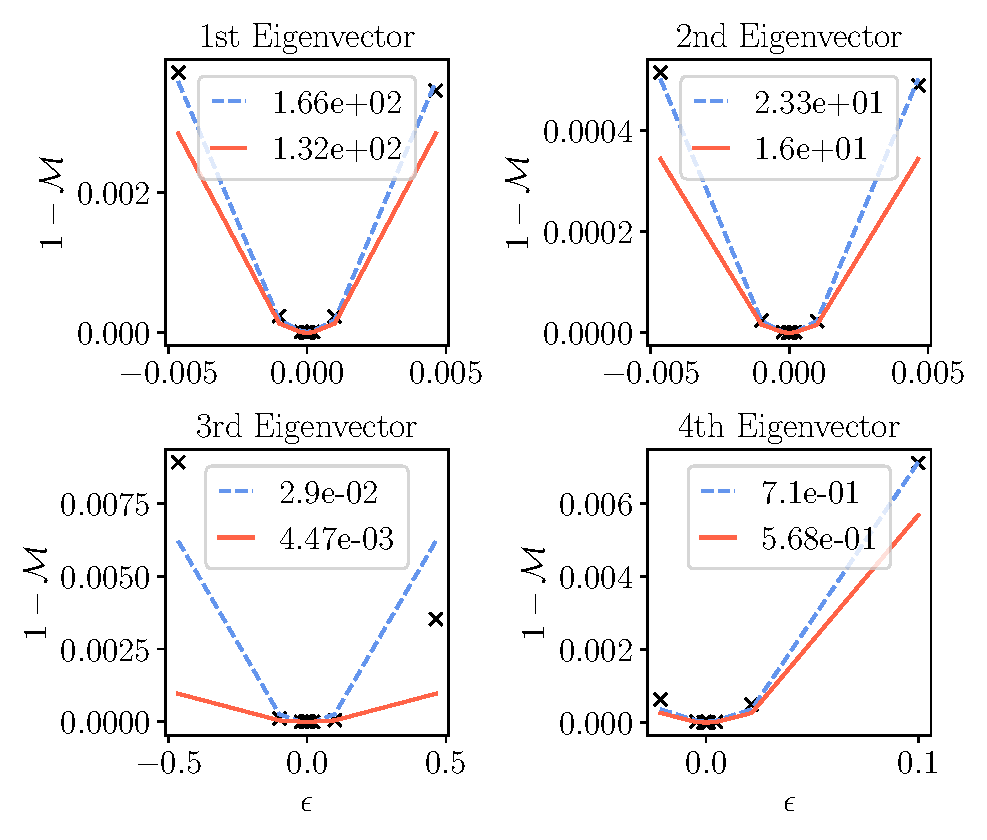
\includegraphics[scale = .52]{parabolae}
	\caption{For each eigenvector of the metric, we compute the empirical relation between the mis-match $1-\mathcal{M}$ and the distance $\epsilon$ of points along the eigenvector direction. The solid line shows the relation predicted by the metric, while the dashed line shows a parabolic fit. In the legend are reported the quadratic coefficients of both lines.}
	\label{fig:parabolae}
\end{figure}

Throughout this paper, we identified the metric with the Hessian of the overlap (see Eq.~\eqref{eq:metric_expression}). While this is widely usd in the literature and has been proven to provide reliable template banks, it still has some non desiderable properties.
To show this, we compute the metric at point $\theta_0 = [20, 3., 0.7, 1.8]$ of manifold \texttt{Mq\_s1xz}, described in Sec.~\ref{sec:placing_accuracy}, and we compute its eigenvalues $\alpha^{(i)}$ and eigenvectors $v^{(i)}$ . We then compute the match $\mathcal{M}^{(i)}_\epsilon$ between $\theta_0$ and the point $\theta^{(i)}_\epsilon = \theta_0 + \epsilon v^{(i)}$, located at a distance $\epsilon$ along i-th eigenvector.
Finally, we  compute the coefficient $\alpha$ of the Taylor expansion $1 - \mathcal{M}^{(i)}_\epsilon = \alpha  \epsilon^2$.
$\alpha$ corresponds to the i-th eigenvalue and in principle, it should be close to its value.

In Fig.~\ref{fig:parabolae}, we plot the fitted relation between $1 - \mathcal{M}$ and $\epsilon$ for each eigenvector, as well as the one computed with the metric. In the legend we report the $a$ coefficient (dashed blue line) and the eigenvalue of the metric (solid orange line).
The striking feature we note in the Figure, is that the eigenvalue is consistently smaller than the fitted $a$ coefficient, sometimes by an order of magnitude.
This means that the hessian, which is computed for $\epsilon\rightarrow 0$, is not able to extrapolate the behaviour of $1 - \mathcal{M}(\epsilon)$ even at modestly large value of $\epsilon$: the metric approximation to the match loses its predictivity as a measure of distance.
The problem becomes more severe in high dimensional manifolds.
On the other hand, since the banks generated with the hessian metric show nice coverage, one may argue that the {\it volume} estimate provided by the hessian is still accurate enough for our purposes.

As a way out, we could redefine the matrix $M_{ij}(\theta)$ to a more suitable expression, departing from the Hessian.
The goodness of the metric expression may depend on the application and on the range of validity of the approximation.
The tensor field $M_{ij}(\theta)$ can be computed through an optimization problem, where we minimize the discrepancy between the two quantities in Eq.~\eqref{eq:metric_definition}, encoded into a {\it loss function}.
The loss function depends on the values of the matrix elements $M^\prime_{ij}$:
\begin{equation} \label{eq:loss_function}
	\mathcal{L}_\theta(M^\prime_{ij}) = \hspace{-4em} \int\limits_{\hspace{3em}\{d(\theta,\theta^\prime) < d_\mathrm{target}\}} \hspace{-3.8em}
		\dvol{\theta^\prime}{D}  \left[ 1 - \mathcal{M}(\theta,\theta^\prime) - M^\prime_{ij} \Delta\theta_i \Delta\theta_j \right]^2
\end{equation}
where the integration extends on a D-ball with radius $d_\mathrm{target}$ centered around $\theta$ and $d_\mathrm{target}$ is a tunable parameter, which controls the validity of the approximation.

At any given point $\theta$, the components $M_{ij}(\theta)$ of the metric are selected by minimizing the above loss:
\begin{equation} \label{eq:metric_optmization}
	M_{ij}(\theta) = \argmin_{M^\prime_{ij}}  \mathcal{L}_\theta(M^\prime_{ij})
\end{equation}
Although the minimization can be tackled with standard techniques, it requires many evaluations of Eq.~\eqref{eq:distance} and sampling from a ``complex" set such as ${\{d(\theta,\theta^\prime) < d_\mathrm{target}\}}$: in most cases this may prove unfeasible.
Future work may try to tackle this optimization problem finding a solution at a feasible computational cost: this may be beneficial to many data analysis applications, such as template placement and Fisher information matrix studies.
A number of alternative metric expression, coming from different heuristic optimization strategies, are already available in \texttt{mbank}, although not fully validated.

	%%%%%%%%%%%%%%%%%%%%%%%%%%%%%%%%% BIBLIOGRAPHY
	\bibliography{biblio.bib}
	\bibliographystyle{ieeetr}

\end{document}



